\documentclass[a4paper,fleqn,usenatbib]{mnras}
\usepackage[T1]{fontenc}
\usepackage{ae,aecompl}


\usepackage{graphicx}	% Including figure files
\usepackage{amsmath}	% Advanced maths commands
\usepackage{amssymb}	% Extra maths symbols
\usepackage{subfig}
\usepackage{array}


\usepackage{multirow}
\usepackage{multicol}
\usepackage{blindtext}
\newcolumntype{?}{!{\vrule width 1pt}}
\newcommand{\Mpch}{\,{\rm Mpc}\,\ifmmode h^{-1}\else $h^{-1}$\fi}
\newcommand{\kpch}{\,{\rm kpc}\,\ifmmode h^{-1}\else $h^{-1}$\fi}
\newcommand{\kpc}{\,{\rm kpc}\,}


\newenvironment{Table}
   {\par\bigskip\noindent\minipage{\columnwidth}\centering}
   {\endminipage\par\bigskip}

\title[Dark Matter halo shape in the AURIGA simulations]{The shape of dark matter
  halos in the AURIGA simulations}  
\author[Jesus Prada,  Jaime E. Forero-Romero, Volker Springel ]{
Jesus Prada,$^{1}$\thanks{E-mail: jd.prada1760@uniandes.edu.co}
Jaime E. Forero-Romero,$^{1}$
Volker Springel$^{2}$
\\
% List of institutions
$^{1}$Departamento de F\'sica, Universidad de los Andes, Cra. 1 No.
18A-10, Edificio Ip, Bogot\', Colombia.\\
$^{2}$Heidelberg Institute for Theoretical Studies, Schloss-Wolfsbrunnenweg 35, D-69118 Heidelberg
Germany.\\
}

% These dates will be filled out by the publisher
\date{Accepted XXX. Received YYY; in original form ZZZ}

% Enter the current year, for the copyright statements etc.
\pubyear{2018}

% Don't change these lines
\begin{document}
\label{firstpage}
\pagerange{\pageref{firstpage}--\pageref{lastpage}}
\maketitle

% Abstract of the paper
\begin{abstract}
We measure the shape of the dark matter halos of Milky Way type galaxies.
\end{abstract}

% Select between one and six entries from the list of approved keywords.
% Don't make up new ones.
\begin{keywords}
keyword1 -- keyword2 -- keyword3
\end{keywords}

%%%%%%%%%%%%%%%%%%%%%%%%%%%%%%%%%%%%%%%%%%%%%%%%%%

%%%%%%%%%%%%%%%%% BODY OF PAPER %%%%%%%%%%%%%%%%%%

\section{Introduction}


A robust prediction of the Cold Dark Matter (CDM) paradigm is that DM
halos are ellipsoidal and can be characterized by the principal axes
$a>b>c$.
This ellipsoidal shape is mostly due to the anisotropical and
clumpy accretion of matter influenced by environmental structures.
Numerical studies how that the shape has a strong mass dependence
\citep{Allgood_et_al._2006}, halos are also rounder at the outerskirts
than at the inner part. 
Shape also evolves with cosmic time, halos get
rounder as they evolve.  

There is however a high degree of uncertainty on what is the degree of
uncertainty on the degree of ellipticity of the Milky Way DM halo.
This problem has been addressed both by observations and simulations.
The difficulty in making an observational measurement lies in the
indirect nature of the effect; i.e. the ellipticity can only be
constrained by its effects on quantities such as stellar radial
velocities.
In simulations the uncertainty on predicting the MW DM ellipticity is 
driven by the different physical effects that should be modeled and
its different possible numerical implementations.


Observationally some studies prefer oblate (i.e. a=b>c) configurations at small
distances around $\leq 20$ kpc
\citep[see][]{Law_and_Majewski_2010,Bovy_et_el._2016,Loebman_et_al._2012,Olling_and_Merrifield_2000,Banerjee_and_Chanda_2011} 
and more triaxial and prolate configurations on the outter distances
$\geq 20$ kpc 
\citep[see][]{Vera-Ciro_and_Helmi_2013,Law_and_Majewski_2009,Deg_and_Widrow_2013,Banerjee_and_Chanda_2011}.
However, some  studies are inclined towards prolate configurations even at the inner
parts of the halo \citep[see][]{Bowden_et_al._2016}, and
although it previously seemed that a triaxial DM halo on the
outerskirts would be necessary to fully explain the characterization
of the Sagittarius stream \citep{Law_and_Majewski_2009}, recent studies
questioned this claim by reporting inconsistencies with narrow stellar
streams \citet{Pearson_et_al._2015} or finding that
the relaxation of other constraints may make this claim unnecessary
\citet{Ibata_et_al._2013}. 

In simulations there is strong evidence claiming that the presence of
baryons produces axisymmetrical halos.  
For instance, some studies have shown that the DM halo shape must be
axisymmetrical to ensure the stability of a hydrodynamical disk
embeded in a static DM halo. 
Other have studied this rounding effect by simulating the disk as rigid
potential inside an N-body triaxial DM
halo \cite{Debattista_et_al._2008,Debattista_et_al._2013,Kazantzidis_et_al._2010}
finding that the halo responds to the disk by becoming less triaxial. 

The caveat of the studies mentioned above is that they do not
follow baryons in the whole cosmological context. 
Other studies overcome this limitation by using resimulations 
\citep{Abadi_et_al._2010,Bryan_et_al._2013} finding that the
feeback related to star formation in the disk drives the strenght of
the round effect. 
Recently \cite{2018arXiv180907255C} made a study in a cosmological
simulation to compare the effect of including baryons. They do find,
on average, rounder halo shapes once hydrodynamic effects are
included, but it is uncertain the strenght of this statistical effect
on galaxies similar to the MW.


All these difficulties (enough numerical resolution, explicit
cosmological context, appropriate feedback physics to produce
realistic MW disks) have limited the studies that want to study the
rounding effect of baryons in MW-like galaxies.
In this work we overcome all these limitations by analyzing the
results of state-of-the-art hydrodynamical simulations of isolated
halos that resemble the Milky Way.
We also perform a convergence study with simulation performed at
different resolution levels and explicitly compare the role of DM only
vs. DM+hydro on the MW DM halo shape.


%\begin{multicols}{2}
\begin{table*}
%\setlength{\tabcolsep}{3pt}
\begin{tabular}{|l|cc|cc|c|c|p{4cm}|}\hline
Reference&$q_{\rho}$&$s_{\rho}$&$q_{\phi}$&$s_{\phi}$&$R$&$\theta$&comment\\ \hline \hline
\citet{Olling_and_Merrifield_2000}& $\mathbf{1.00}$ & $\mathbf{0.80}$ & & & $\simeq 8$kpc & $0^{\circ}$&Method: Stellar dynamics and HI density. \\\hline
\citet{Law_and_Majewski_2009}&&&$\mathbf{0.83}$&$\mathbf{0.67}$& $\lesssim 60$kpc&$90^{\circ}$&Mid-axis orientation. Method: Sagittarius stream\\\hline
%
\citet{Law_and_Majewski_2010}&&&$\mathbf{0.99}$&$\mathbf{0.72}$& $[20$kpc,$60$kpc$]$&$90^{\circ}$&Mid-axis orientation, Method: Sagittarius stream\\\hline
%
\citet{Loebman_et_al._2012}&$\mathbf{1.00}$&$\mathbf{0.47}$&&&$\sim 20$kpc &$0^{\circ}$&Method: SDSS statistics\\\hline
%
\citet{Deg_and_Widrow_2013}&$0.72$&$0.28$&$0.82$&$0.40$&$[20$kpc,$60$kpc$]$&$90^{\circ}$& Mid-axis orientation. Method: Sagittarius stream\\\hline
%
\multirow{2}{*}{\citet{Vera-Ciro_and_Helmi_2013}}&&&$\mathbf{1.00}$&$\mathbf{0.90}$&$\lesssim 10$kpc&$0^{\circ}$ & Method: Sagittarius stream \& LMC \\
&&&$\mathbf{0.90}$&$\mathbf{0.80}$&$\gtrsim 10$kpc&$90^{\circ}$& Mid-axis orientation on the outside. \\\hline
%
\citet{Bovy_et_el._2016}&$\mathbf{0.95}$&$\mathbf{0.95}$&&&$\lesssim 20$kpc&$90^{\circ}$ & Method: Stellar streams\\\hline
%
\citet{Bowden_et_al._2016}&&&$\mathbf{[0.5,0.66]}$&$\mathbf{[0.5,0.66]}$&$[5$kpc,$10$kpc$]$&$90^{\circ}$& Weak constraint on prolate halo. Method: SDSS stars dynamics.\\\hline
%
\multirow{2}{*}{\citet{Banerjee_and_Chanda_2011}}&$\mathbf{1}$&$\mathbf{1}$&&&$9$kpc&$0^{\circ}$&Method: HI gas. \\
&$\mathbf{0.5}$&$\mathbf{0.5}$&&&$24$kpc&$0^{\circ}$&Monotonical change between radial regimes.\\\hline
%
\cite{Johnston_et_al._2005}&$\mathbf{1}$&$\mathbf{[0.83-0.92]}$&&&$\lesssim 60$kpc&$0^{\circ}$&Method: Sagittarius stream\\\hline\hline
\end{tabular}
\caption{(TODO: compute analogues in isopotential or isodensity according to Binney and Tremaine)}
\end{table*}
%\end{multicols}

\begin{table*}
%\setlength{\tabcolsep}{3pt}
\begin{tabular}{|l|cc|cc|c|p{4cm}|}\hline
Reference&$q_{\rho}$&$s_{\rho}$&$q_{\phi}$&$s_{\phi}$&$R$&comment\\ \hline \hline
\citet{Chua_et_al._2018}&$\mathbf{0.88\pm0.10}$&$\mathbf{0.70\pm0.11}$&&&$0.15R_{200}$& Illustris\\\hline
%
\citet{Bryan_et_al._2013}&$\mathbf{[0.84,0.86]}$&$\mathbf{[0.66,0.70]}$&&&$R_{200}$& For different cosmologies and feedback recipies. Calculated from a fit at $M_\odot=10^12$\\\hline
%
\multirow{2}{*}{\citet{Abadi_et_al._2010}}&&&$\mathbf{0.98}$&$\mathbf{0.85}$&-& Almost independent of radius. No feedback: boundary case\\\hline
\end{tabular}
\caption{(TODO: compute analogues in isopotential or isodensity according to Binney and Tremaine)}
\end{table*}




\section{Numerical Simulations}

In this work we use the results of the state-of-the art Auriga
simulations \citep{auriga}. 
The objects in those simulations were selected from a set of 30
isolated halos in the Evolution and Assembly of GaLaxies and their
Environments (EAGLE)  project \citep{Eagle}.   
These halos were randomly selected from a sample of the most isolated
halos whose virial mass $M_{200}$ varied between $10^{12}M_\odot$ and
$2\times 10^{12}M_\odot$. 
These halos were re-simulated with higher resolution an varying
physical realism using the AREPO code \citep{arepo}.
 
All 30 halos were simulated within resolution defined for Aquarius
simulations corresponding to $\sim 3\times 10^6$ high resolution DM
particles of $\sim 2.5 \times 10^5 M_\odot$.  
This resolution is labeled as Level 4, the main details for each halo
are consigned in Table \ref{tab:level4}. 
From these 30 halos, 6 of them where re-simulated at higher resolution
(labeled as Level 3) taking into account a spatial factor of 2 in each
dimension.   
Details of Level 3 halos are in Table \ref{tab:level3}. 
Furthermore, for each halo in each level of resolution there are two
versions of the simulation: DM-only and DM plus baryons with
magneto-hydrodynamical (MHD) physics.  

\begin{table*}
\centering
\begin{tabular}{l|cc|cc|cc|cc}
\hline
\hline
Halo & \multicolumn{2}{c}{$N_P$/$10^6$} & \multicolumn{2}{c}{$M_P$/$10^5M_\odot$} & 
\multicolumn{2}{c}{$R_{vir}$/kpc} & \multicolumn{2}{c}{$M_{vir}$/$10^{14} M_\odot$}  \\ \hline
& DM & MHD& DM & MHD& DM & MHD& DM & MHD\\ \hline \hline
halo 1&4.068&2.447&2.397&2.022&196.927&187.674&9.062&7.844\\
halo 2&5.625&5.457&2.481&2.093&235.094&233.934&15.418&15.191\\
halo 3&3.826&3.852&2.645&2.231&210.693&210.955&11.099&11.141\\
halo 4&4.585&4.530&2.590&2.185&219.378&215.438&12.529&11.866\\
halo 5&3.262&3.290&2.533&2.137&196.984&197.246&9.071&9.106\\ 
halo 6 ($\star$)&3.184&3.110&2.337&1.972&191.840&189.342&8.378&8.054\\ 
halo 7&3.878&3.729&2.296&1.937&197.864&196.509&9.193&9.005\\
halo 8&2.772&2.796&2.451&2.068&190.716&191.764&8.231&8.368\\
halo 9&3.038&3.010&2.738&2.310&195.826&190.640&8.911&8.222\\
halo 10&2.700&2.751&2.541&2.144&187.139&188.147&7.777&7.904\\
halo 11&4.146&4.116&2.541&2.144&221.821&219.568&12.952&12.560\\
halo 12&2.865&2.908&2.645&2.231&192.280&192.038&8.436&8.404\\
halo 13&3.520&3.600&2.393&2.019&202.139&203.815&9.801&10.048\\
halo 14&4.200&4.475&2.499&2.108&215.535&218.927&11.882&12.453\\
halo 15&2.888&2.845&2.541&2.144&199.848&200.658&9.471&9.588\\ 
halo 16 ($\star$)&3.821&3.871&2.499&2.108&212.590&212.632&11.401&11.408\\ 
halo 17&2.752&2.781&2.552&2.153&188.067&187.404&7.893&7.811\\
halo 18&3.770&3.624&2.738&2.310&201.124&207.293&9.655&10.571\\
halo 19&2.989&3.086&2.645&2.231&200.244&200.325&9.527&9.540\\
halo 20&3.903&3.822&2.481&2.093&210.097&211.423&11.005&11.214\\ 
halo 21 ($\star$) &4.105&4.075&2.640&2.227&219.527&219.823&12.555&12.604\\ 
halo 22&2.794&2.766&2.625&2.215&188.363&184.801&7.931&7.489\\ 
halo 23 ($\star$) &3.977&4.073&2.795&2.358&217.768&215.959&12.254&11.952\\
halo 24 ($\star$) &4.466&4.426&2.522&2.127&217.440&215.147&12.199&11.817\\ 
halo 25&2.902&2.806&2.645&2.231&199.922&198.299&9.482&9.254\\
halo 26 &4.610&4.716&2.506&2.115&219.984&218.939&12.633&12.454\\
halo 27 ($\star$) & 5.060&5.018&2.590&2.185&228.036&226.225&14.071&13.740\\ 
halo 28 & 4.184&4.276&2.645&2.231&216.979&217.997&12.121&12.294\\
halo 29 & 4.827&4.613&2.499&2.108&225.791&219.935&13.660&12.625\\
halo 30 & 3.268&3.112&2.579&2.176&195.043&194.741&8.805&8.763\\
\hline
\hline
\end{tabular}
\caption{Specifications of each level 4 galaxy (halo). 
  The DM and MHD versions of each parameters are presented together. 
  The columns correspond to: (1) Halo name, (2,3) Millions of DM
  particles belonging to the halo, (4,5) DM particle mass in
  $10^5M_\odot$, (6,7) Halo Virial radius in kpc and (8,9) halo virial
  mass in $10^{14}M_\odot$. Halos marked with a star ($\star$) are
  correspond to halos resimulated at higher resolution (level 3).}  
\label{tab:level4}
\end{table*} 

\begin{table*}
\centering
\begin{tabular}{l?cc?cc?cc?cc}
\hline
\hline
Halo & \multicolumn{2}{c?}{$N_P$/$10^6$} & \multicolumn{2}{c?}{$M_P$/$10^5M_\odot$} & \multicolumn{2}{c?}{$R_{vir}$/kpc}&\multicolumn{2}{c}{$M_{vir}$/$10^{14}M_\odot$}  \\ \hline
& DM & MHD& DM & MHD& DM & MHD& DM & MHD\\ \hline \hline
halo 6&24.902&24.185&0.292&0.246&191.741&188.367&8.365&7.932\\
halo 16&29.750&30.334&0.312&0.263&212.622&212.542&11.406&11.395\\
halo 21&31.993&31.503&0.330&0.278&219.731&220.250&12.588&12.679\\
halo 23&31.379&31.618&0.349&0.295&217.793&213.358&12.259&11.524\\
halo 24&34.987&35.153&0.315&0.266&217.313&213.963&12.179&11.624\\
halo 27&39.617&39.056&0.324&0.273&227.908&223.484&14.048&13.244\\
\hline
\hline
\end{tabular}
\caption{Same layout Table \ref{tab:level3} for Level 3 simulations (higher
  resolution than Level 4 simulations).}
\label{tab:level3}
\end{table*} 

\section{Determining the halo shape}

%\subsection{The solid ellipsoid method}

The DM halo shape at a fixed radius is an estimate of either
the isopotential or isodensity surfaces.  
Observational inference models usually estimate the 
isopotential contours which are probed by tracers (gas, stars), while
simulations work with the isodensity contours which can be directly
calculated from particle positions.  

However, in numerical simulations the density contours are not smooth
and are sensitive to the presence of small satelites. 
For this reason we choose to measure the shape by taking
volume-enclosed particles, rather than shell-enclosed.  
We follow the shape measurement method presented by
\cite{Allgood_et_al._2006} that uses the reduced
inertia tensor,     

\begin{equation}
I_{ij} = \sum_k \frac{x_k^{(i)}x_k^{(j)}}{d^2_k},
\label{eq:inertia}
\end{equation}

with the positions components weighted by the k-th particle distance
$d_k^2=x_k^2+y_k^2+z_k^2$, the particle positions are measured from
the minimum of the gravitational potential in each halo.
The diagonalization of this tensor yields the principal axes of the
structure as well as the eigen-quantities which are proportional to
the squared principal axes $a>b>c$. 

We start the calculations taking into account particles within a
sphere of radius $R$ and then  recharacterize the triaxial parameters
by taking into account particles within an ellipsoid of semi-axes
$r,r/q,r/s$ and re-scaled distance $d^2=x^2+(y/q)^2+(z/s)^2$, where $q
= b/a$ and $s=c/a$ are the previously calculated axial ratios. 
We repeat this process until the average deviation of semi-axes is
less than $10^{-6}$.  
This is the same method used to estimate the halo shape in the DM-only
Aquarius simulations \citep{Vera-Ciro_et_al._2011}. 

We restrict the sampling of the ellipsoidal parameters to radii
between $1/16 R_{vir}$ and $2R_{vir}$, where  $R_{vir}$ is taken as the
radius enclosing a sphere with 500 times the average dark matter
density of the Universe. 
All our results use of this reference radius
unless strictly stated otherwise. 
We peform the shape measurements both as a function of radius and
redshift for all halos in the sample.


\section{Results}

\subsection{Radial trends at $z=0$}

\begin{figure*}
  \centering
  \subfloat[halo 27 DM shape at small
    radius]{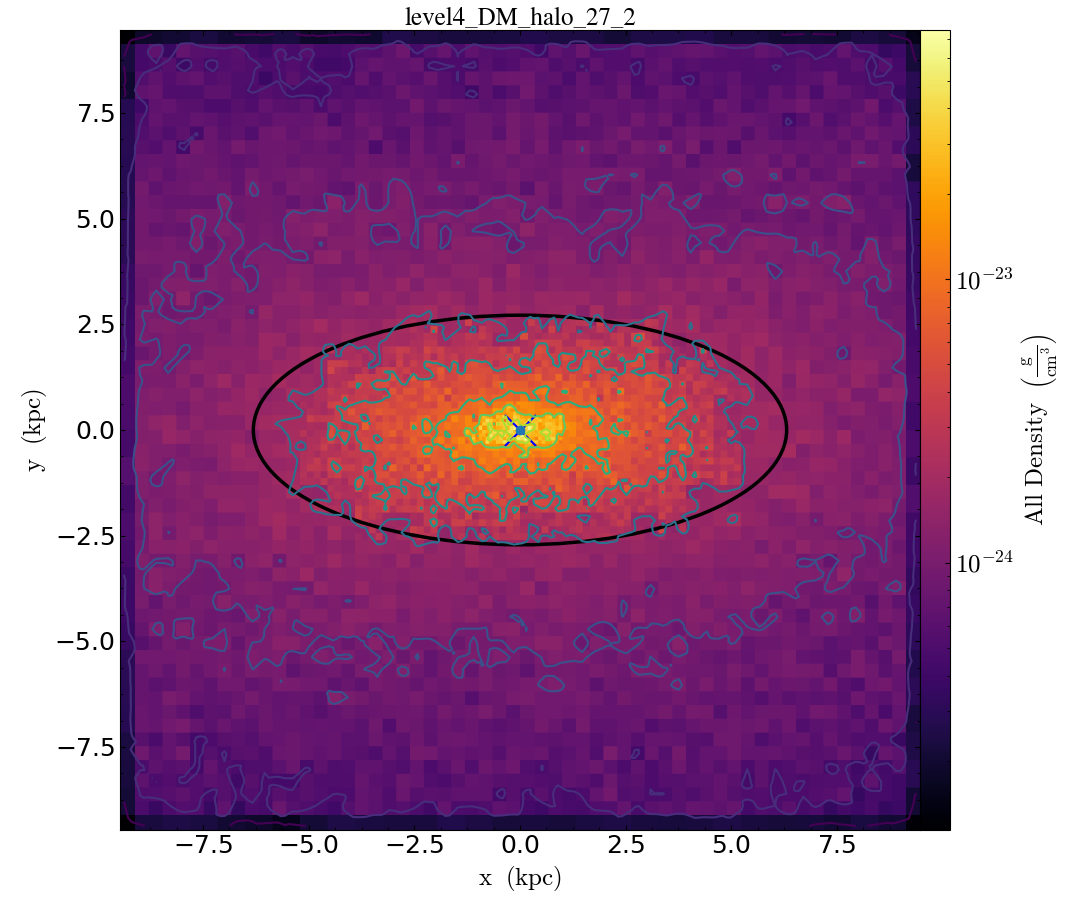
\includegraphics[width=0.5\textwidth]{./pics/MHD_Vs_DM/level4_DM_halo_27_inner.png}} 
  \hfill
  \subfloat[halo 27 DM shape at big
    radius]{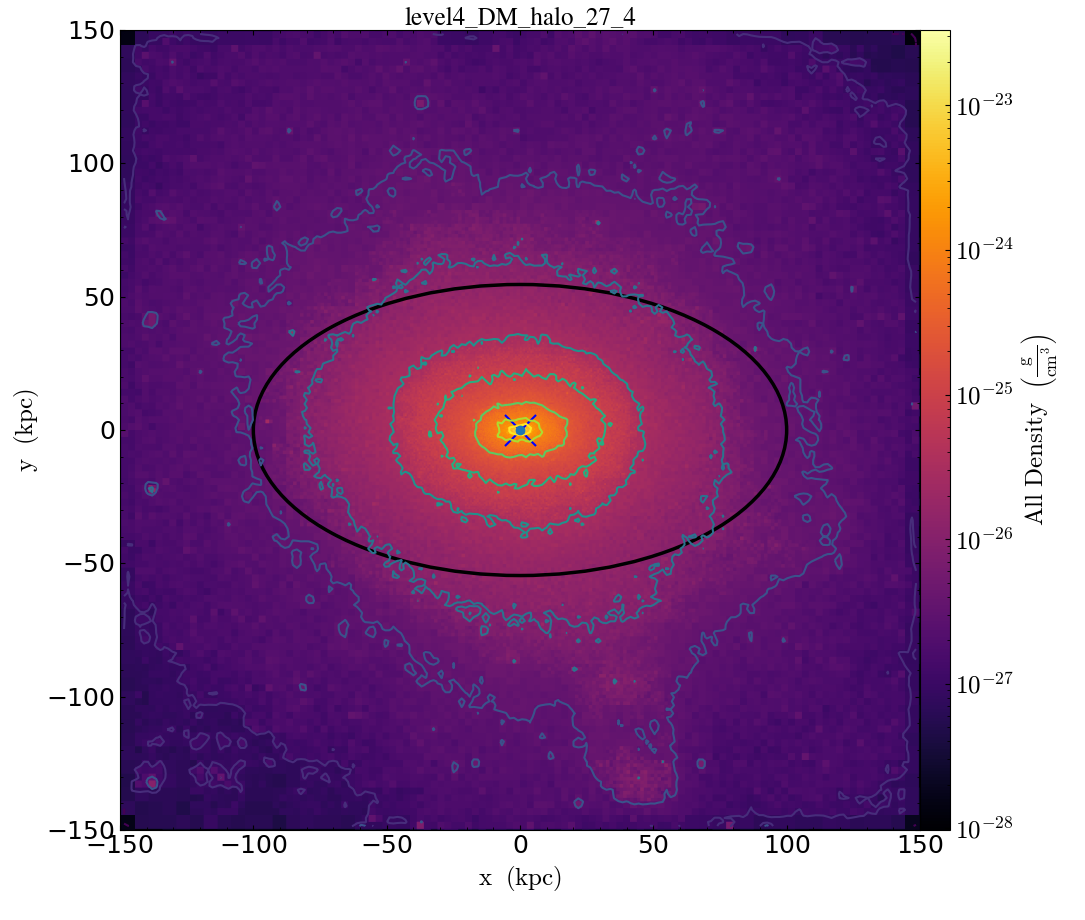
\includegraphics[width=0.5\textwidth]{./pics/MHD_Vs_DM/level4_DM_halo_27_outter.png}} 
  \hfill 
  \caption{DM density for inner/outer (left/right panel) DM halo regions.  
  Slice 20 percent of the max-min range in the "z" position of
  particles belonging to the main structure, centered at halo defined
  position (calculated with most bounded particle) }  
  \label{fig:slices}
\end{figure*}

We find that in DM-only simulations halos are monotonically rounder
with increasing radius, confirming results already reported in the
literature \citep{Vera-Ciro_et_al._2011}. 
Figure \ref{fig:slices} illustrates this effect.
There we show the density a DM-only halo at redshift zero in a thin
slice passing through the halo's centre, each panel shows the halo at
different radii.
The ellipse plotted over the contours indicates the outermost
boundary of the estimated shape ellipsoid. 
Indeed, the ellipse panel on the right (outer halo) is rounder than
the ellipse on the left (inner halo). 


\begin{figure*}
\centering
{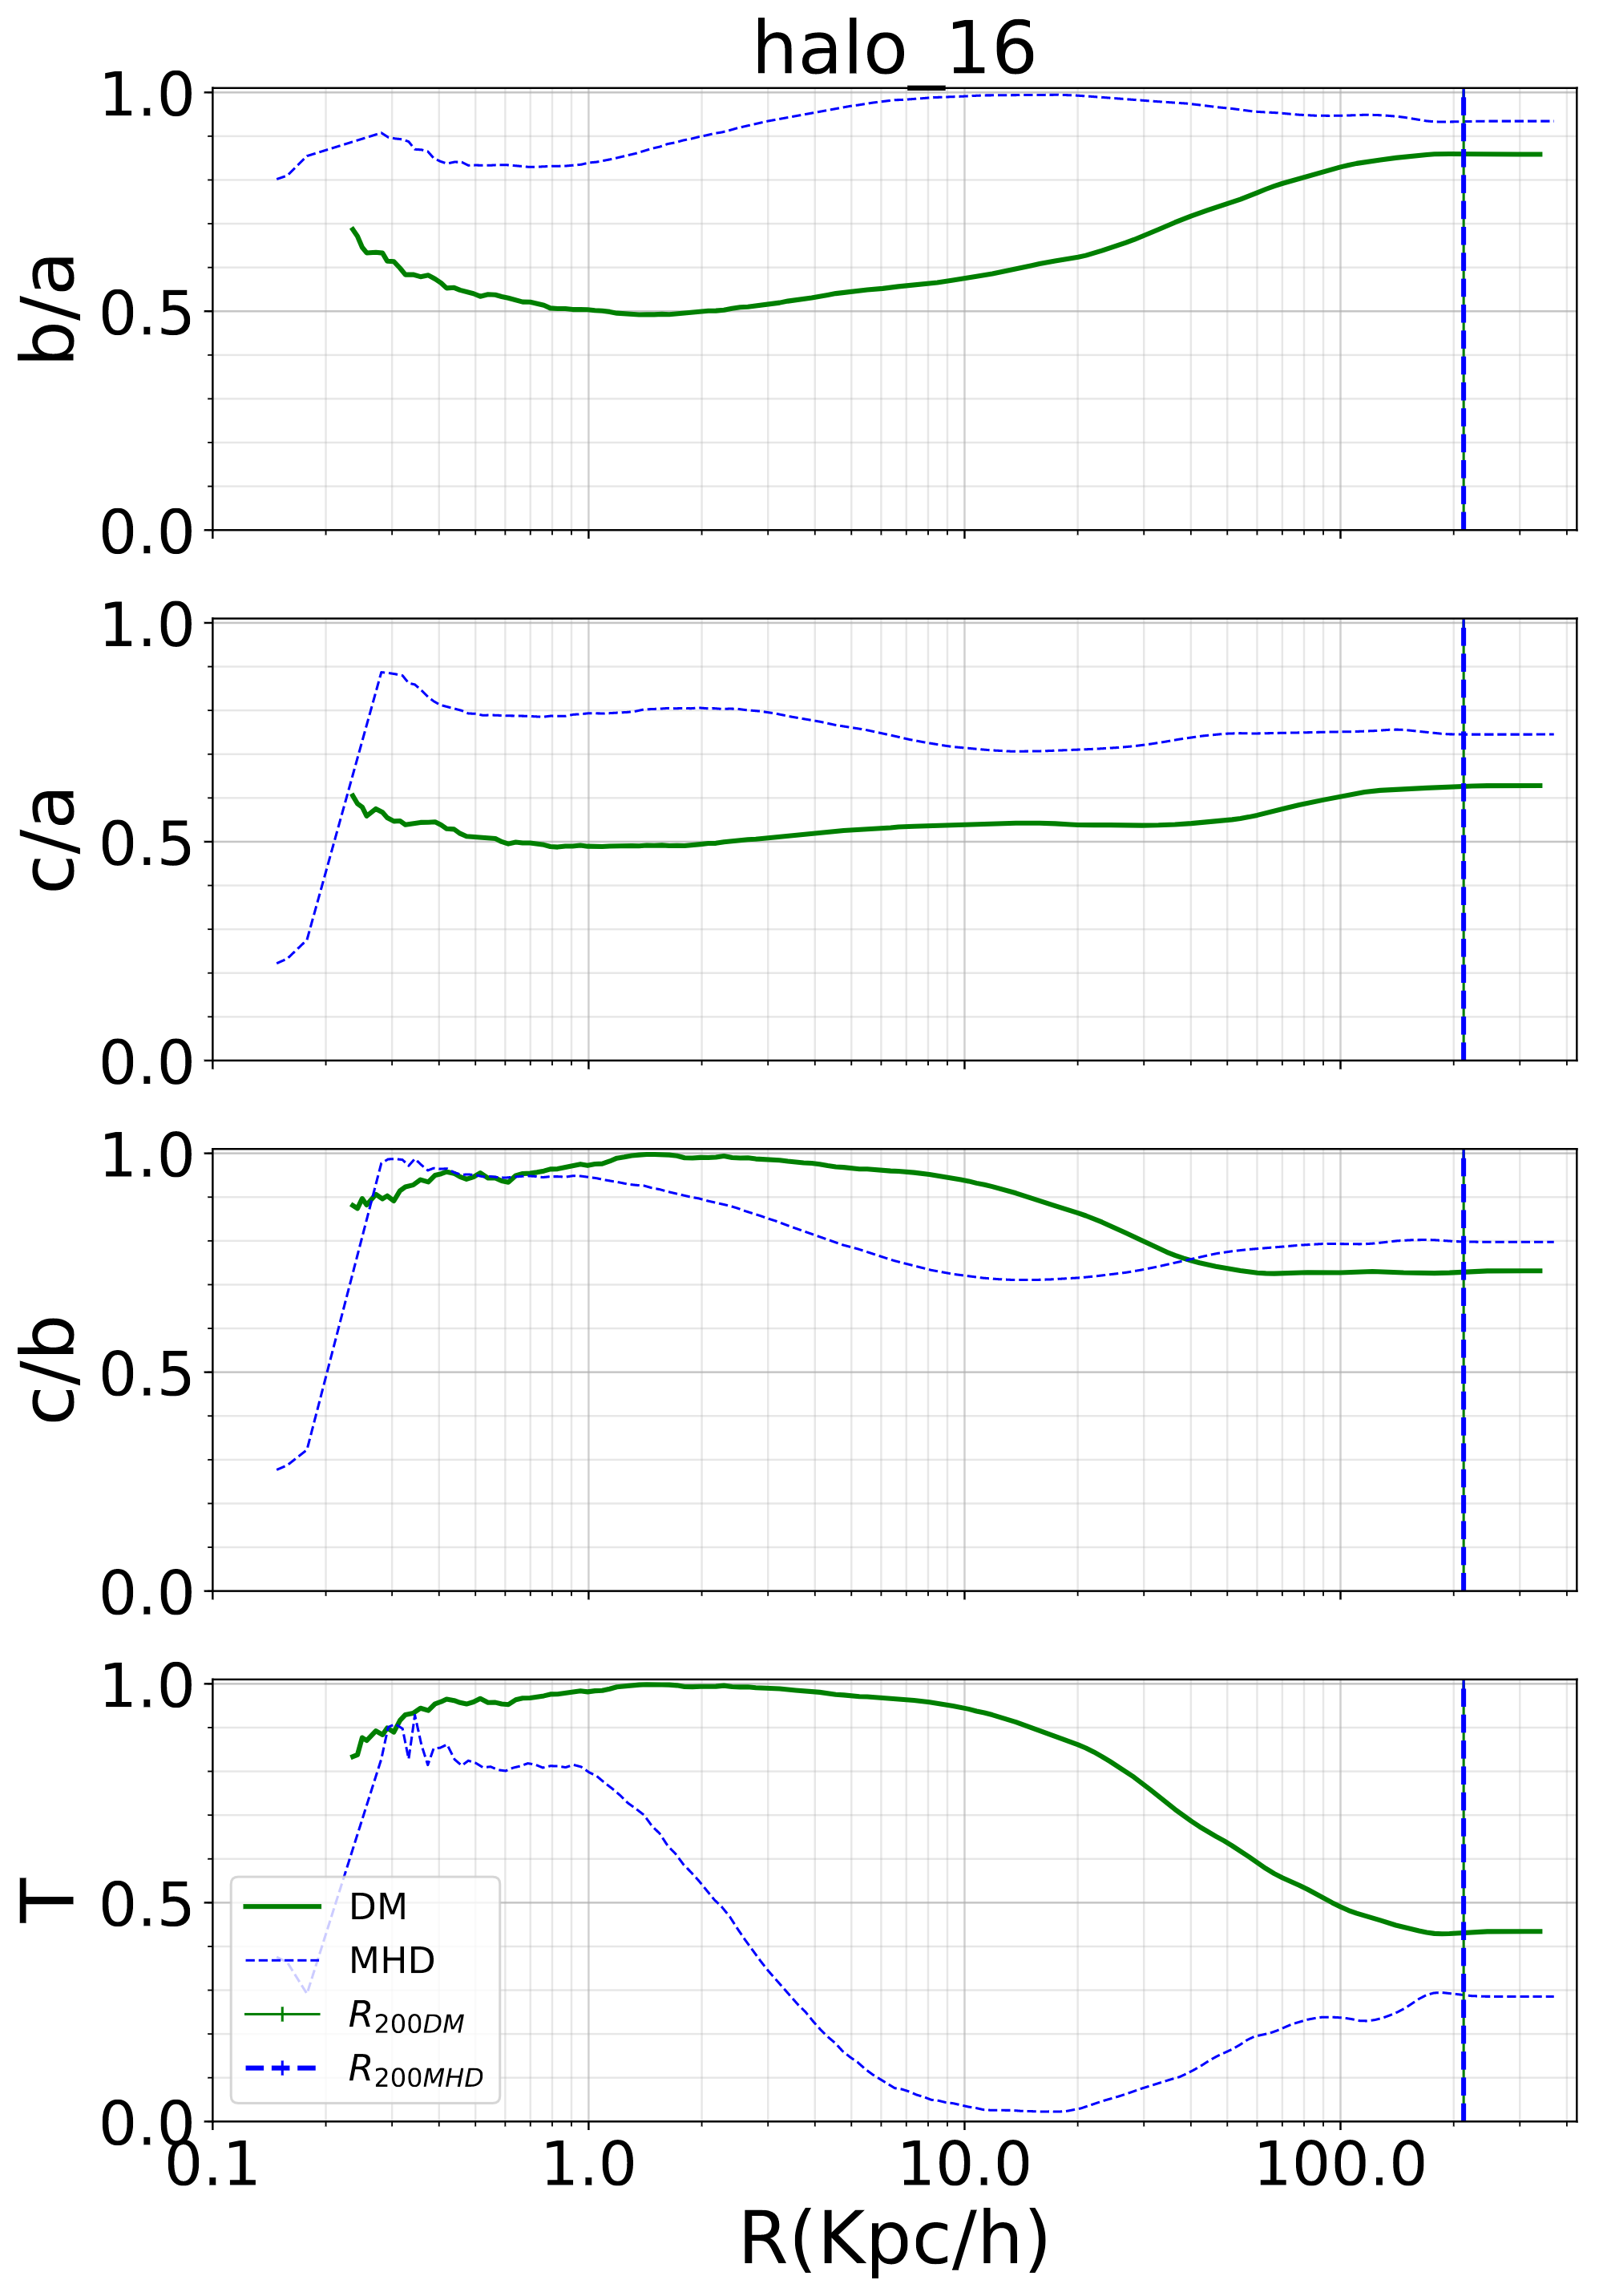
\includegraphics[width=0.6\textwidth]{./pics/halo16.png}}
\caption{Radial profile for the axial ratios and the triaxiality parameter
  $T=\frac{1-b/a}{1-c/a}$ at redshift $z=0$. 
  Radial profile was sampled at
  redshift 0 and there are two sets of lines showing MHD and DM-only
  versions of the axial ratios profile} \label{fig:triaxial_radius}
\end{figure*} 


We quantify this effect by plotting the axial ratios $q$, $s$,
$s/q$ and the triaxiality $T\equiv \frac{1-q}{1-s}$ as a
function of radius. 
As a representative sample of this relations we show on Figure
\ref{fig:triaxial_radius} the radial trends for Halo 16 at
the highest resolution both for DM and MHD simulations.
The continous lines correspond to the DM simulation and shows how
the inner part of the halo $r\approx 1$\kpch has values of 
$q=0.5$, $s=0.5$ while at the virial radius the same
quantities increase to $q=0.85$, $s=0.6$; in turn the triaxiality
decreases from $T\approx 1.0$ to $T\approx0.4$. 

In the same Figure \ref{fig:triaxial_radius} we also find one of the
main results of our study: halos in MHD simulations are systematically rounder, at
every radius, than its DM-only counterparts.  
The dashed line in Figure \ref{fig:triaxial_radius} shows that at
$r\approx 1$\kpch  in the MHD simulation we have $q=0.85, s=0.8$
($q=0.5, s=0.5$ in DM) and at the virial radius $q=0.95, s=0.75$
($q=0.85, s=0.6$ in DM).  
However, the triaxiality trend is not as monotonous for MHD halos is
it is in DM halos. 
The triaxiality goes almost to zero at an intermediate radius,
$r\approx 10$\kpc in the case of Halo 16 in Figure
\ref{fig:triaxial_radius}, to increase again. {\bf pasa lo mismo para
  todos los halos? es lo mismo para baja y alta resolucion de MHD?}
    

Figure \ref{fig:triax_DM} summarizes this comparizon for all 30 halos
in the Level 3 simulations. 
Measurements at $R_{\rm vir}/16$ are represented by circles while squares 
are measurements at $R_{\rm vir}$. 
All halos, except two, show that outer regions rounder than inner
regions.
The exceptions are cases where a merging substructures near  the
halo's center gives rise to perturbed axial ratio measurements. 
Figure \ref{fig:triax_MHD} shows the same information, this time for
the MHD simulations. 
In this case, the main radial trend continues to hold, albeit less
pronounced.
We also find that halos in MHD simulations are in general rounder than
their DM counterparts

This average behaviour of more round halos in MHD can be seen more
clearly in the individual case of Halo 16, shown in Figure
\ref{fig:triaxial_radius}.  
At the virial radius the halo is rounder than its DM counterpart. 
Going from the virial radius to $10$ \kpch the $b/a$ ratio is constant almost close to unity
in the MHD simulation while it decreases to $0.5$ in DM-only
simulation. 
Between $2$-$10$ \kpc the triaxiality in the DM-only simulation is in
the range $0.9-1.0$, while the MHD simulation has values between
$0-0.5$. 


In Table \ref{table:median_axial_ratio_DM} and Table \ref{table:median_axial_ratio_MHD}
we summarize these trends for the median values of the axis ratio in
the two sets of simulations (DM and MHD). 
The lower/upper bounds correspond to the first/third quartiles. 
Summarizing: a) Table  \ref{table:median_axial_ratio_DM} shows how halos are
monotonically rounder with increasing radius; b) the comparison
against Table \ref{table:median_axial_ratio_MHD} shows  how DM halos
are consistently rounder in MHD simulations than DM-only runs at every radius.


 
\begin{figure}
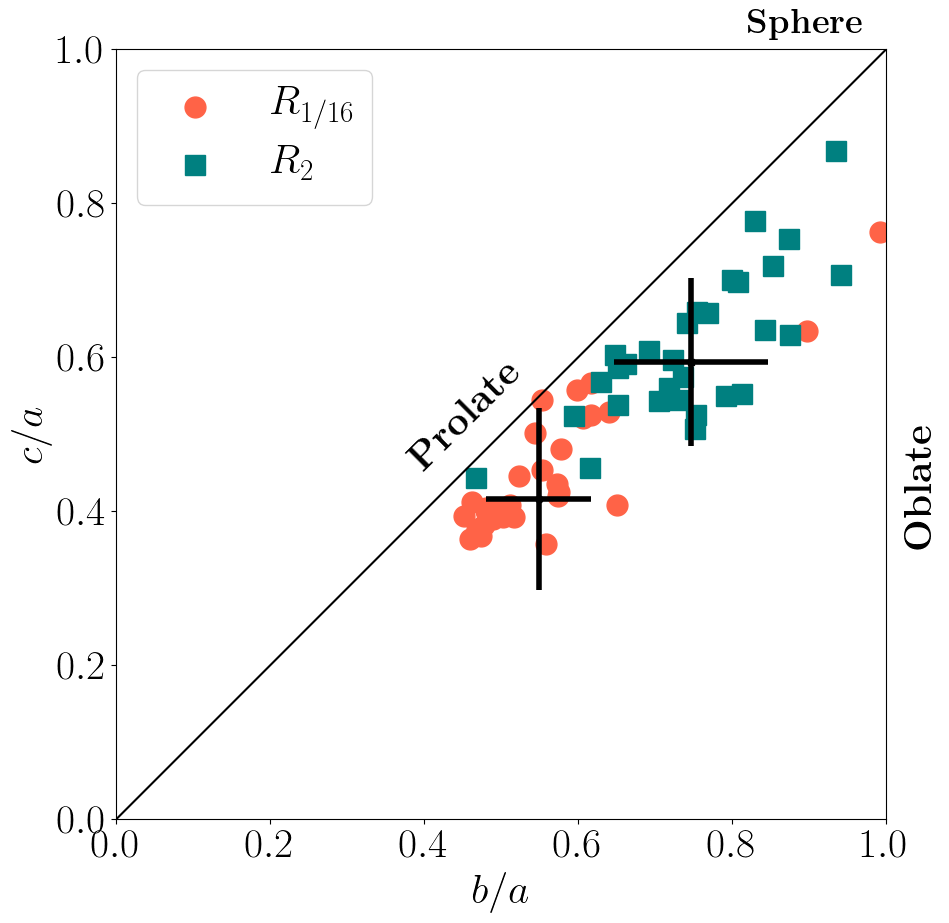
\includegraphics[width=0.9\columnwidth]{./pics/Triaxial_Plane/Triax_DM.png}
\caption{Axial ratios for the 30 halos in the Level 3 DM simulations.
   Each dot represents the shape characterization of each halo at the 2 times the virial radius and a  1/16 fraction of the virial radius differentiated by color.
  Errorbar shows median and errors for each sampled radii.
  Conclusion: DM halos are rounder on the outskirts {\bf Esto necesita
  correccion. Debe ser a R1/16 y R (no 2R!)}}
  \label{fig:triax_DM}
\end{figure}


\begin{figure}
 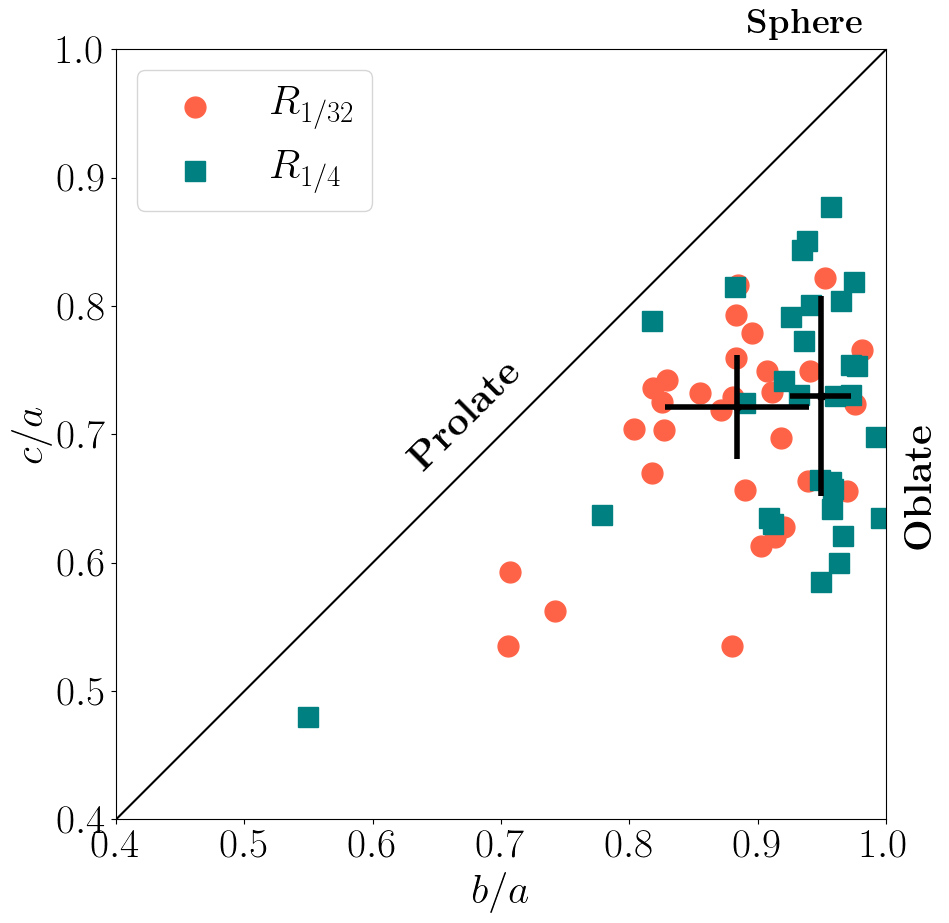
\includegraphics[width=0.9\columnwidth]{./pics/Triaxial_Plane/Triax_MHD.png}
  \caption{Axial ratios for the 30 halos in the Level 3 MHD
    simulations. DM halos are rounder at larger radii than small radii. {\bf Esto
      necesita correccion para que tambien sea a 
      R1/16 y R.}}
  \label{fig:triax_MHD}
\end{figure}



\begin{table}
\setlength{\tabcolsep}{3pt}
\begin{center}
\begin{tabular}{l|ccccc}
 &$R_{1/16}$& $R_{1/8}$& $R_{1/4}$& $R_{1/2}$& $R_1$\\
\hline 
$b/a$ &$0.55^{+0.07}_{-0.07}$&$0.57^{+0.09}_{-0.08}$&$0.61^{+0.15}_{-0.08}$&$0.65^{+0.18}_{-0.10}$&$0.70^{+0.13}_{-0.10}$ \\ [0.1cm]
$c/a$ &$0.42^{+0.12}_{-0.03}$&$0.45^{+0.11}_{-0.04}$&$0.49^{+0.09}_{-0.05}$&$0.52^{+0.10}_{-0.05}$&$0.56^{+0.10}_{-0.05}$\\ [0.1cm]
$T$ &$0.89^{+0.03}_{-0.08}$&$0.88^{+0.04}_{-0.12}$&$0.84^{+0.08}_{-0.23}$&$0.81^{+0.08}_{-0.29}$&$0.75^{+0.14}_{-0.25}$\\ [0.1cm]
\end{tabular}
\end{center}
\caption{Median values of axial ratios $q,s$ and triaxiality parameter
  $T$ for DM halos in DM-only simulations at different radii. The
  median is computed over the 30 halos in Level 3 simulations.}  
\label{table:median_axial_ratio_DM}
\end{table}



\begin{table}
\setlength{\tabcolsep}{3pt}
\begin{center}
\begin{tabular}{l|ccccc}
 &$R_{1/16}$& $R_{1/8}$& $R_{1/4}$& $R_{1/2}$& $R_1$\\
\hline 
$b/a$ &$0.93^{+0.04}_{-0.04}$&$0.95^{+0.03}_{-0.03}$&$0.95^{+0.02}_{-0.05}$&$0.93^{+0.04}_{-0.06}$&$0.93^{+0.04}_{-0.10}$\\[0.1cm]
$c/a$ &$0.73^{+0.05}_{-0.09}$&$0.73^{+0.07}_{-0.10}$&$0.73^{+0.08}_{-0.10}$&$0.73^{+0.09}_{-0.08}$&$0.75^{+0.07}_{-0.11}$\\[0.1cm] 
$T$ &$0.31^{+0.15}_{-0.22}$&$0.20^{+0.24}_{-0.12}$&$0.24^{+0.20}_{-0.12}$&$0.30^{+0.26}_{-0.16}$&$0.36^{+0.23}_{-0.23}$\\[0.1cm] 
\end{tabular}
\end{center}
\caption{Median values of axial ratios $q,s$ and triaxiality parameter
  $T$ for DM halos in MHD-only simulations at different radii. The
  median is computed over the 30 halos in Level 3 simulations.}  
\label{table:median_axial_ratio_MHD}
\end{table}




\subsection{The historical shape}
One of the principal motivations to study the radial dependence of the
DM halo shape is that it may encode some clues about its formation
history. We have already shown that DM-only halos seem to exhibit a
steady and monotonous growth in its axial ratios when sampled at
bigger radii. One similar effect can be found if we sample the shape
at the virial radius, this time at varying redshift. It is easy to see
that the axial ratios increase with decreasing redshift, which is
expected by the continuous influence of the gravitational potential
\cite{Vera-Ciro_et_al._2011}. In figure \ref{fig:RedshiftGood} we
present a representative example.
 
\begin{figure}
  \subfloat[halo 16 DM]{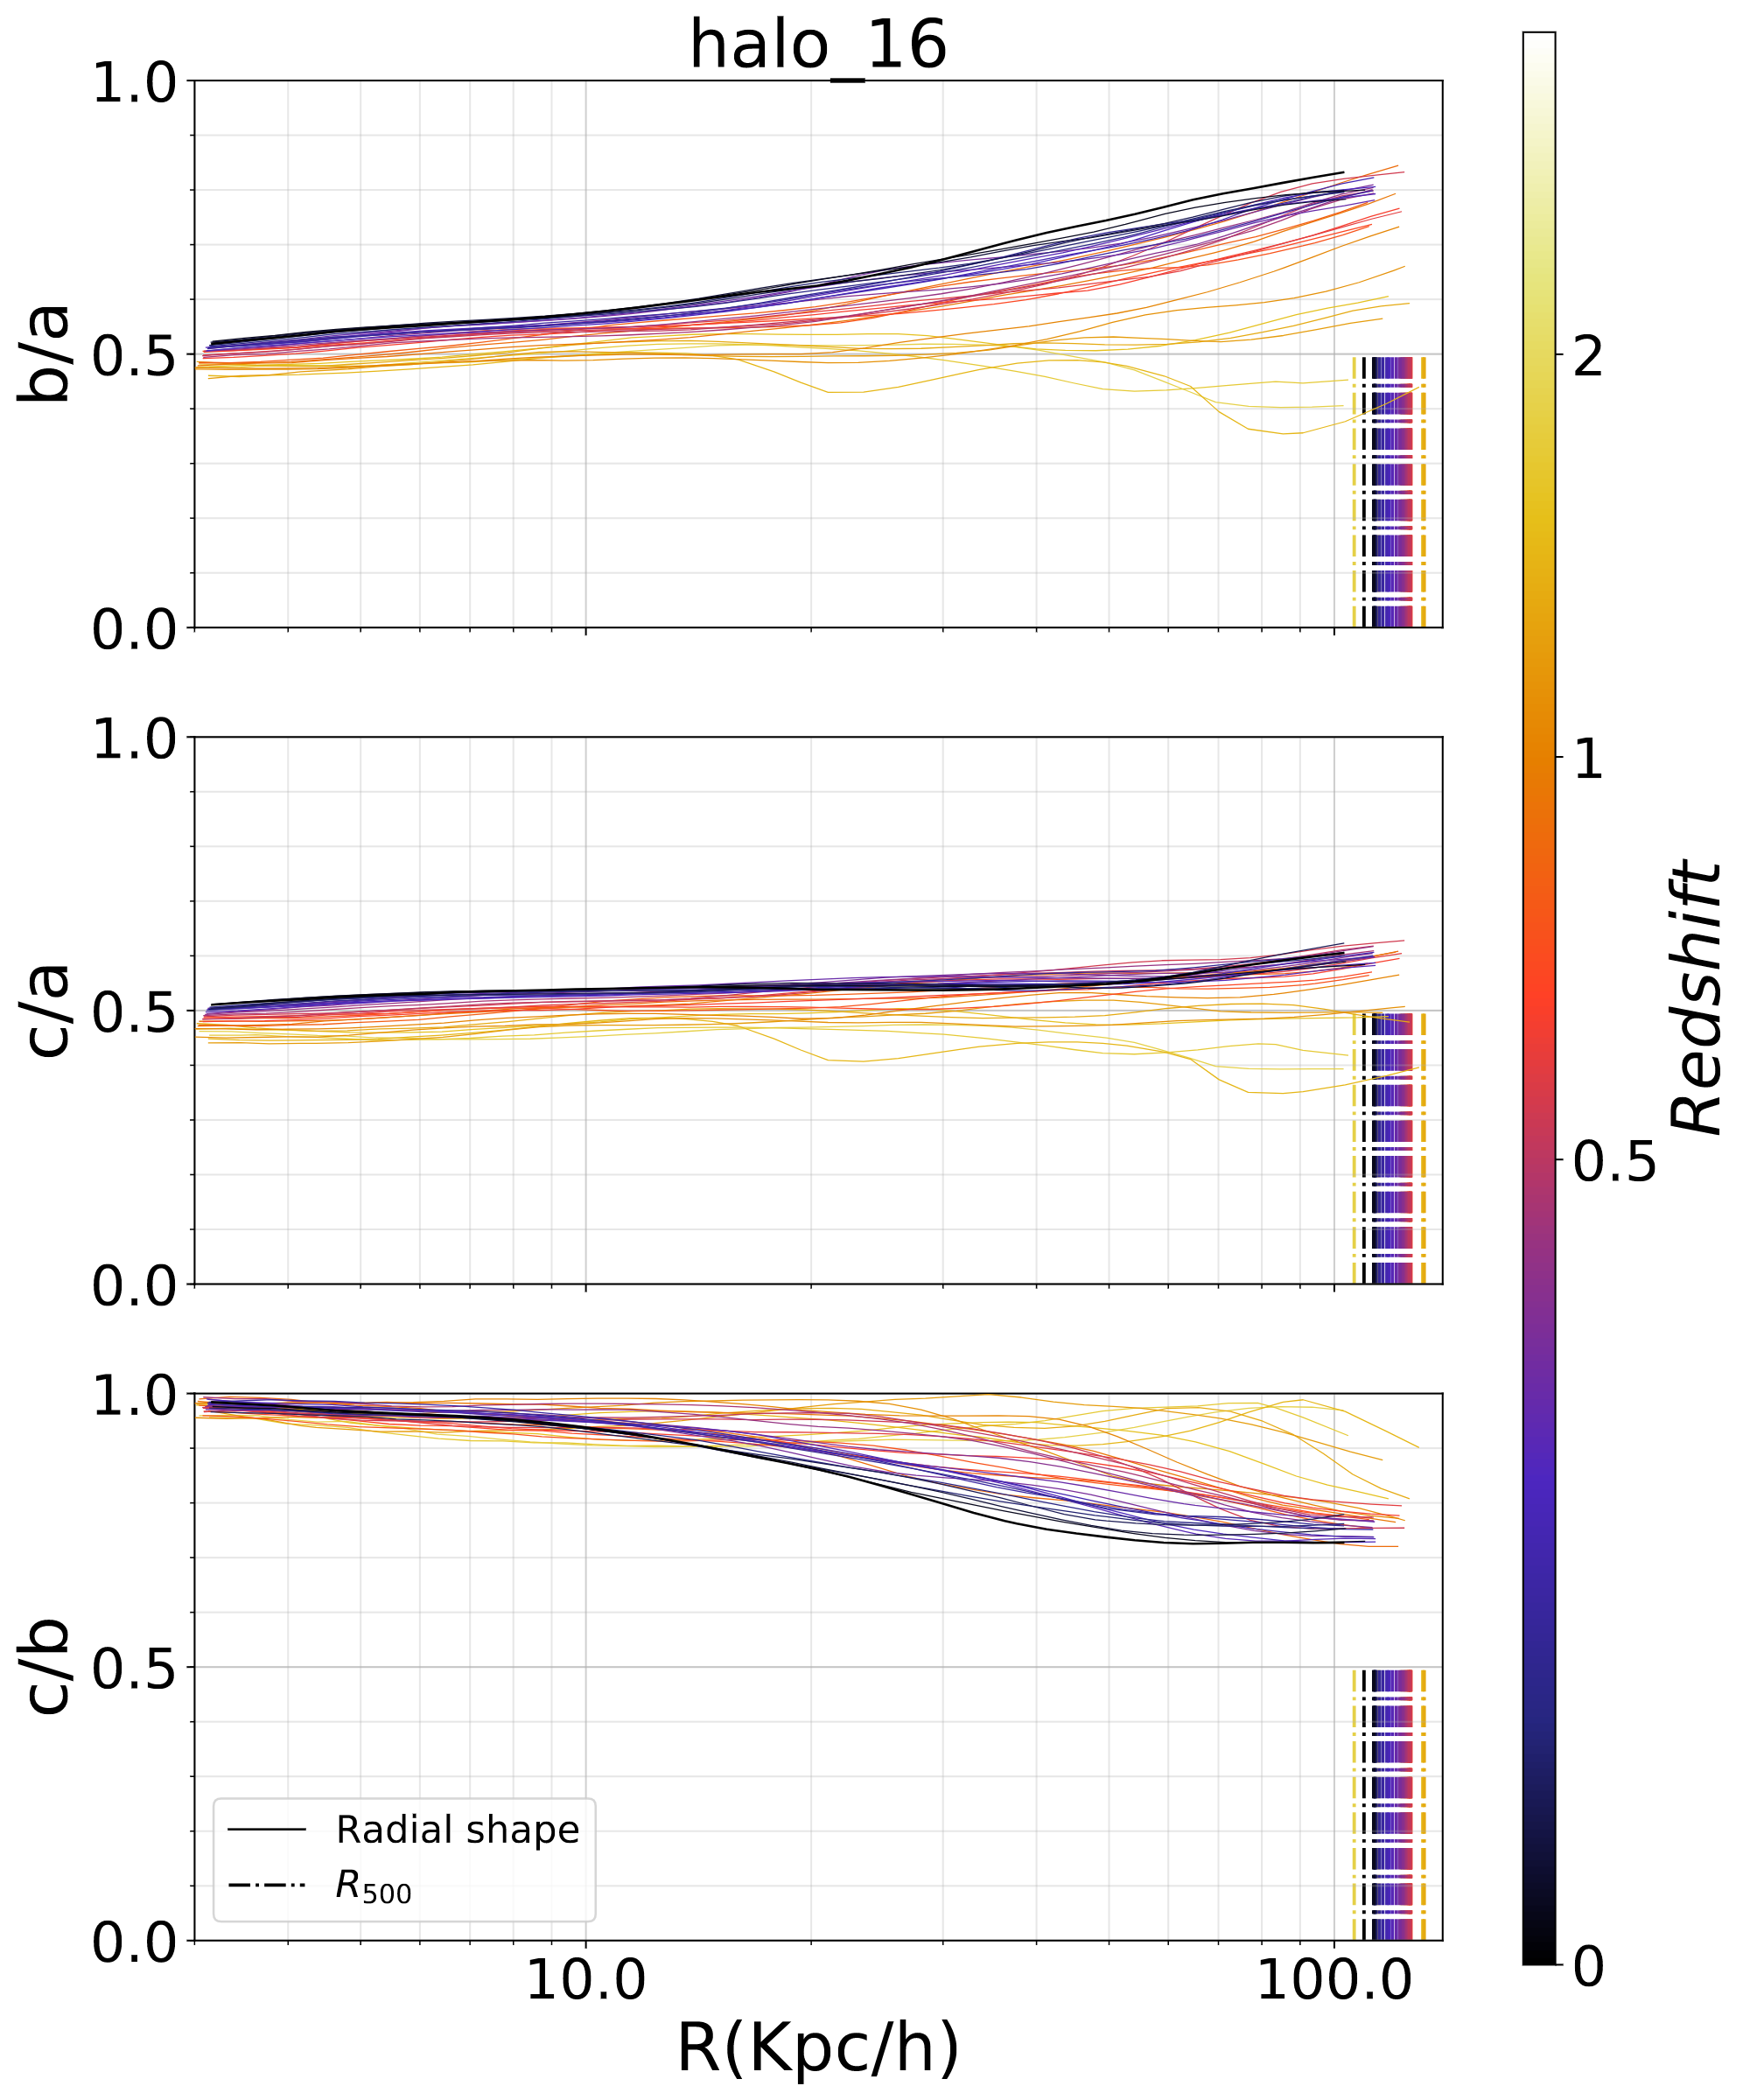
\includegraphics[width=0.5\columnwidth]{./pics/Redshift/halo_16_level3_DM_Z.png}}
  \subfloat[halo 16 MHD]{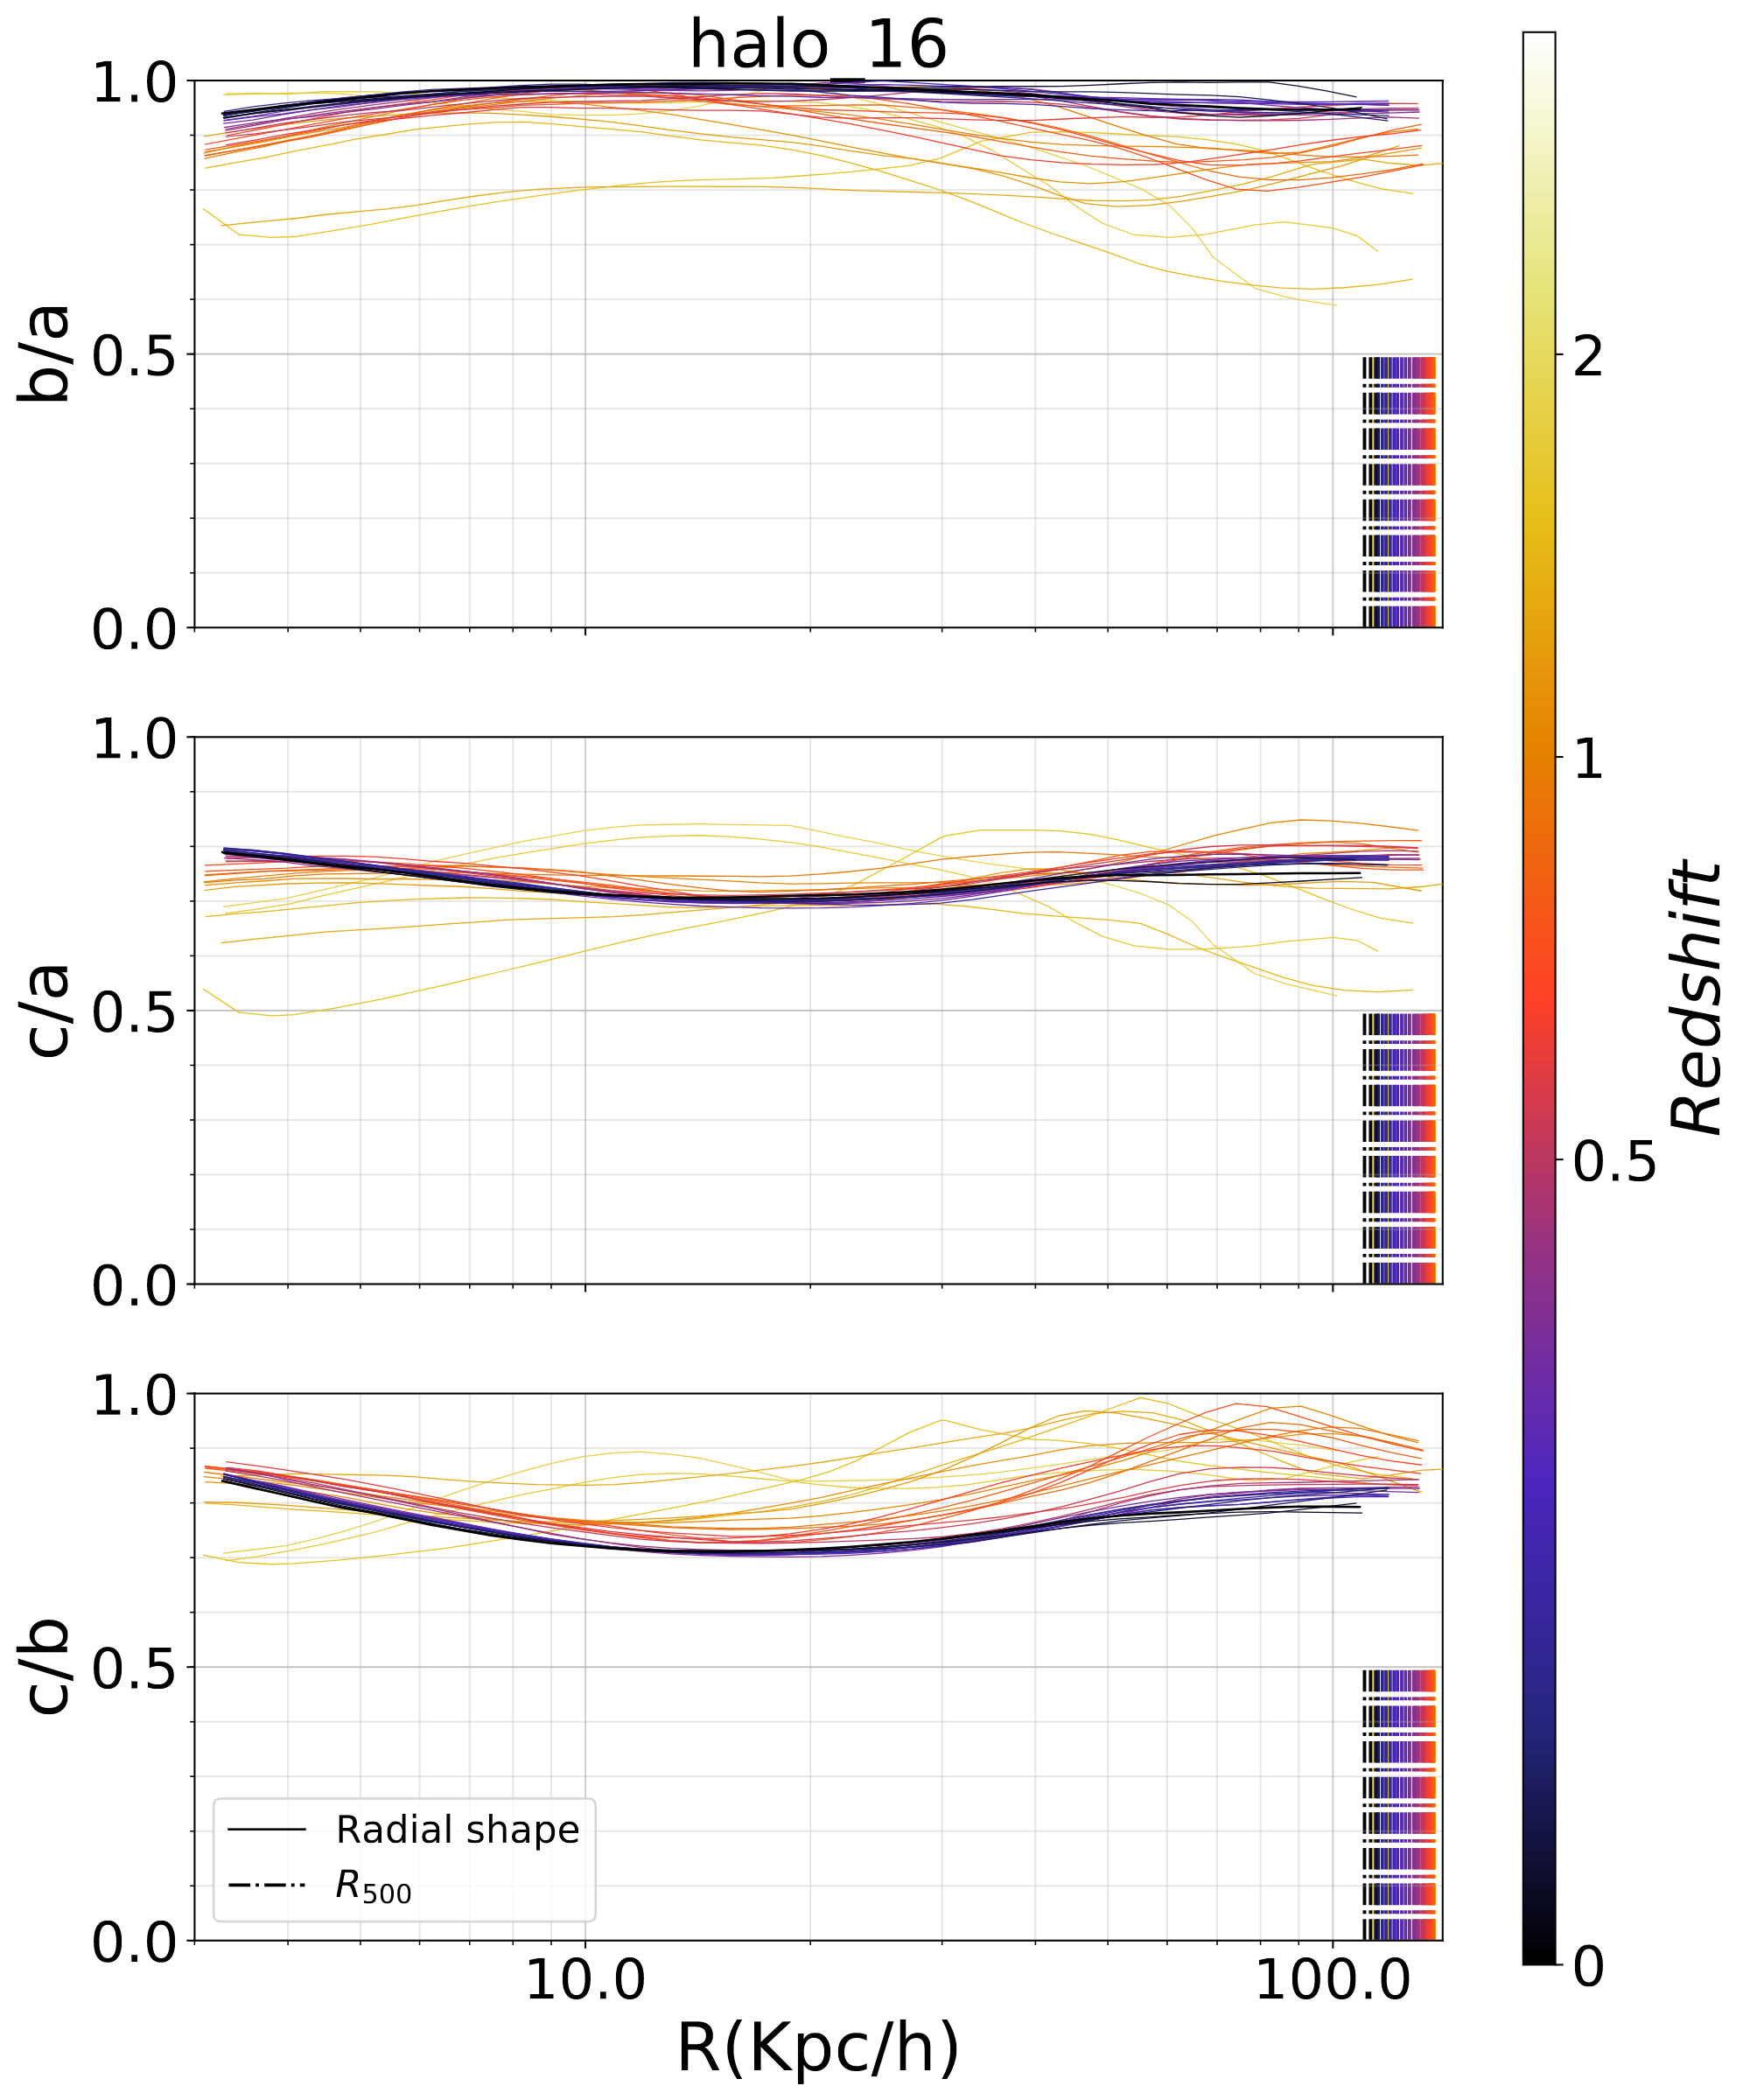
\includegraphics[width=0.5\columnwidth]{./pics/Redshift/halo_16_level3_MHD_Z.png}}
  \caption{Radial profile (comoving) of axial ratios for halo 16 in
    terms of redshift (color). This halo maintains its shape until
    $z\approx 1$ obviating the systematic rounding effect in time from
    asymmetric potentials. Each plot-line represents the radial
    profile at a determined redshift. Conclussion: Mainly for b/a, it increases for:
    (1) for bigger radii (fixed redshift)(2) for lower redshift (fixed
    radius) It explains the correlation between radial profile and
    history, but does not require that curves match in the triaxial
    plane.}
  \label{fig:RedshiftGood}
\end{figure}


Interestingly, these two parametic plots i.e. $(b/a,c/a)(z=0,r)$ and
$(b/a,c/a)(z,r=R_{vir})$ are very correlated for DM-only halos
\ref{fig:DM Z Triax}. This means that, for DM-only halos, one can
approximate its shape at higher redshift by simply sampling its
current shape at a smaller radius \textbf{wording}. This relationship
relies strongly on the steady and monotonous tendency of DM halos
towards sphericity for bigger radii and smaller redshift. 


\begin{figure}
  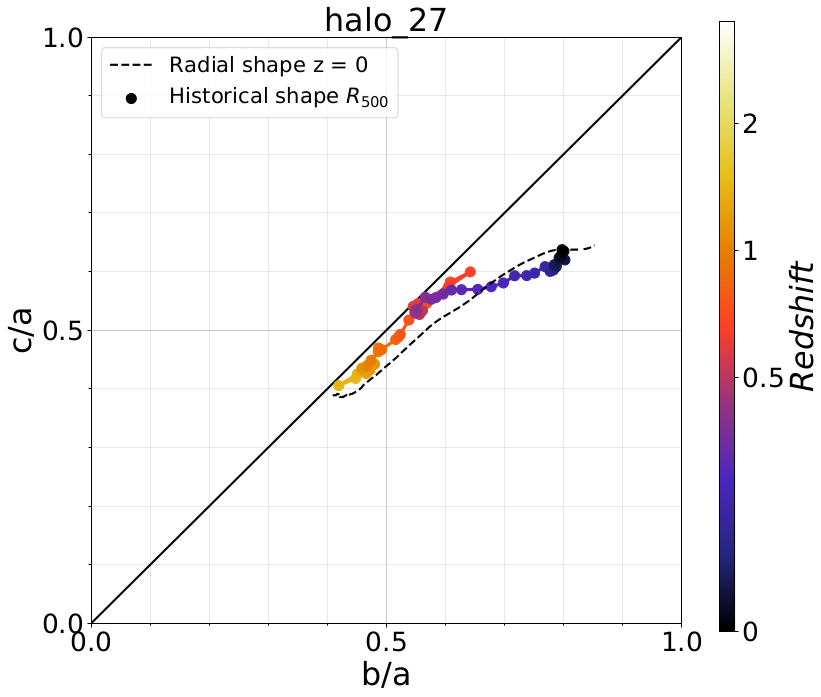
\includegraphics[width=\columnwidth]{./pics/Redshift/halo_27_DM_Z_correlation.png}
  \caption{DM only Radial profile at redshift 0 (dashed line)
    Historical profile at virial radius R500 (colour line). Example
    of a halo where there is some correlation between these two
    profiles, as usually happens for DM only
    simulations. Conclusion: DM only halos usually (fraction?) have
    correlated shape profiles.} 
  \label{fig:DM Z Triax}
\end{figure}

MHD halos, on the other hand, do not exhibit tendency towards
sphericity with bigger radii, but they do get sistematically rounder
at lower redshift as seen in figure \ref{fig:RedshiftGood}. This
effectively vanishes this correlation as seen from a DM halo
\ref{fig:MHD Z Triax}. 

\begin{figure}
  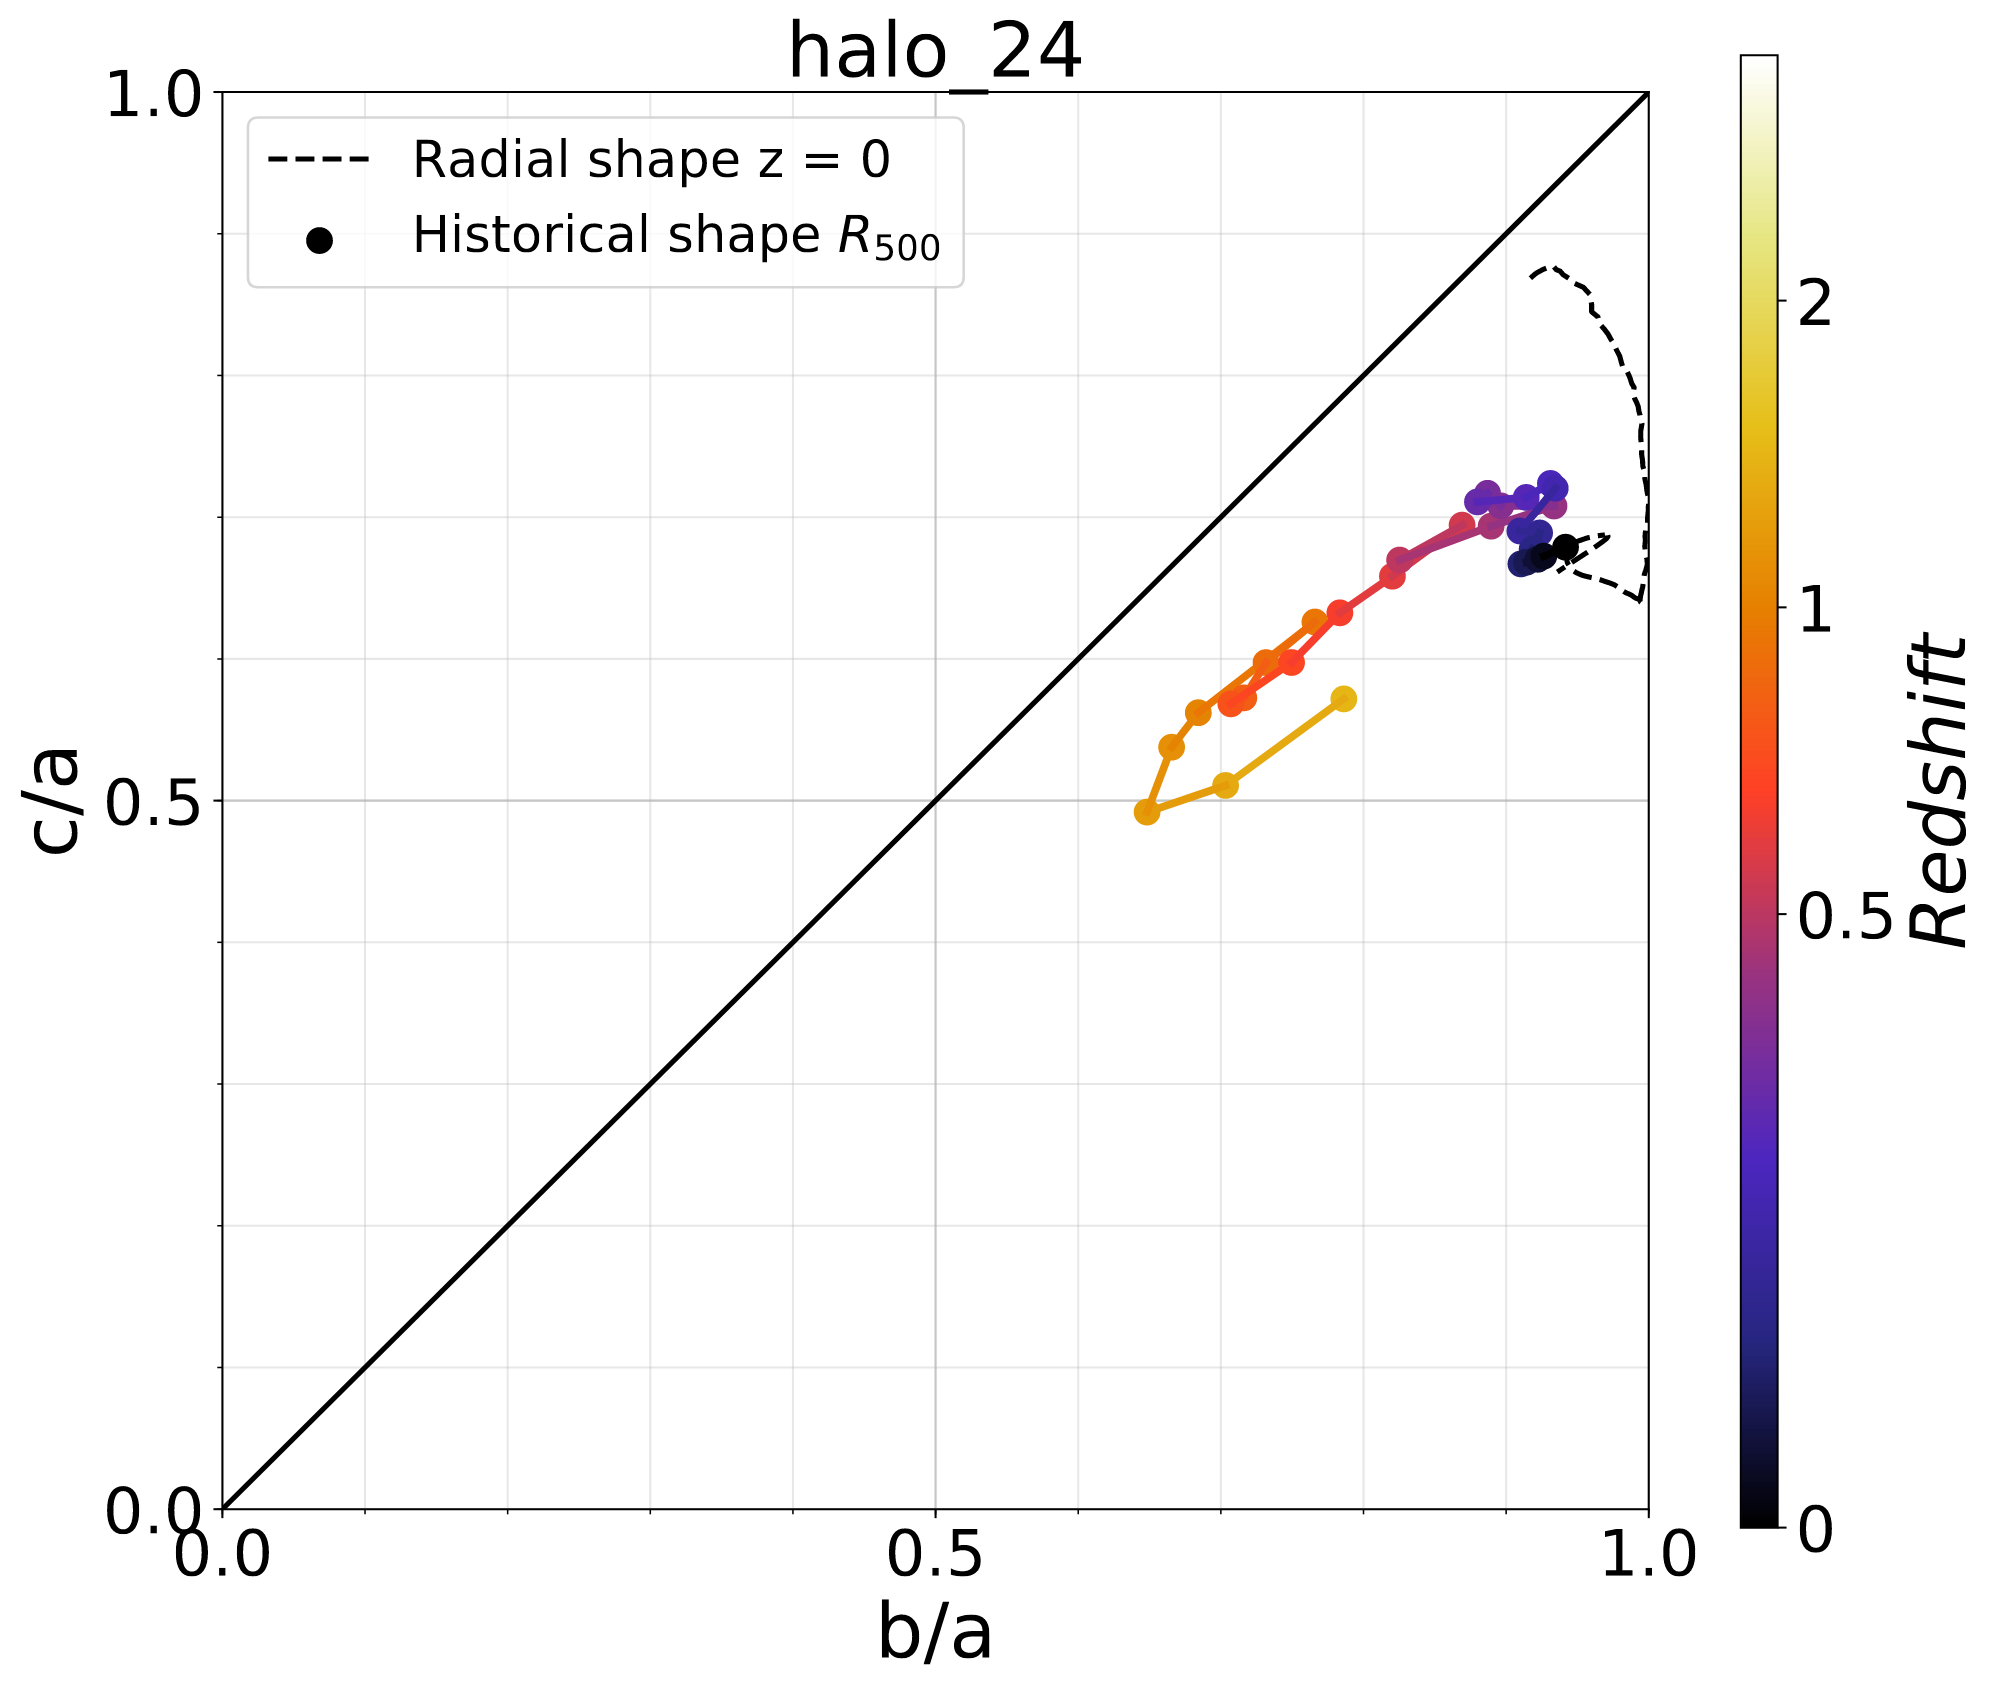
\includegraphics[width=\columnwidth]{./pics/Redshift/halo_24_level3_MHD_Z_Triax.png}
  \caption{MHD. Radial profile at redshift 0 (dashed line)
    Historical profile at virial radius R500 (colour line)
    Example of a halo where there is no correlation
    between these two profiles, as usually happens in
    MHD. Conclusion: MHD halos usually (fraction?) have uncorrelated shape profiles.}
    \label{fig:MHD Z Triax} 
\end{figure}

Better graphics.

%Discuss if this correlation may be recovered if compared for example at Disk radius in stead of virial radius.\\


\subsection{The orientation of the principa axes}

One of the principal assumptions of observational models of the MW's
DM halo is that its minor axis is perfectly aligned with the disk
axis. Although this is a reasonable assumption to guarantee the
stability of the galactic disk in simplified models of isolated
galaxies, it may not be the case for galaxies evolved in the whole
cosmological context nor at every radii at which the shape is
sampled. 

Therefore, it is of special interest to us to examin the strength of
this alignment assumption in the context of simulations. For this
purpose, we sampled the shape at 5 different radii and plotted the
axial directions, as well as the disk direction in the \textbf{name}
diagrams \cite{} (explain diagrams). Explain disk direction
calculation. 

We found that there is not a representative example of what happens in
terms of alignments. We found that the majority of the disks are
aligned with the minor axis of their DM halo within $\approx 30^o$; in
some special cases, this alignment was almost perfect and in some
other cases, the DM halo minor axis changed substantially to be able
to determine an alignment. In figure \ref{fig:alignment} we present
these three cases. \textbf{occurrencies for each case?} 


\textit{This is an important result of our study. We study the radial
  evolution of the principal axes, compared also to the angular
  momentum vector from the disk. We found that while the angular
  momentum tend to be aligned with the minor axis of the ellipsoid,
  this may not be the case all times. When there is an alignment it is
  usually within 20 degrees (get a histogram of this. and an evolution
  of this histogram with time). When there is not an alignment, then
  there is no simple way to determine towards which axis it is
  oriented. Furthermore, the principal axes alignment usually change
  with radius (rotation, swap, verify). This ask for relaxation on the
  strong constrains on the MW DM halo models.} 


\begin{figure}
  \centering
  \subfloat[Perfectly aligned Axes]{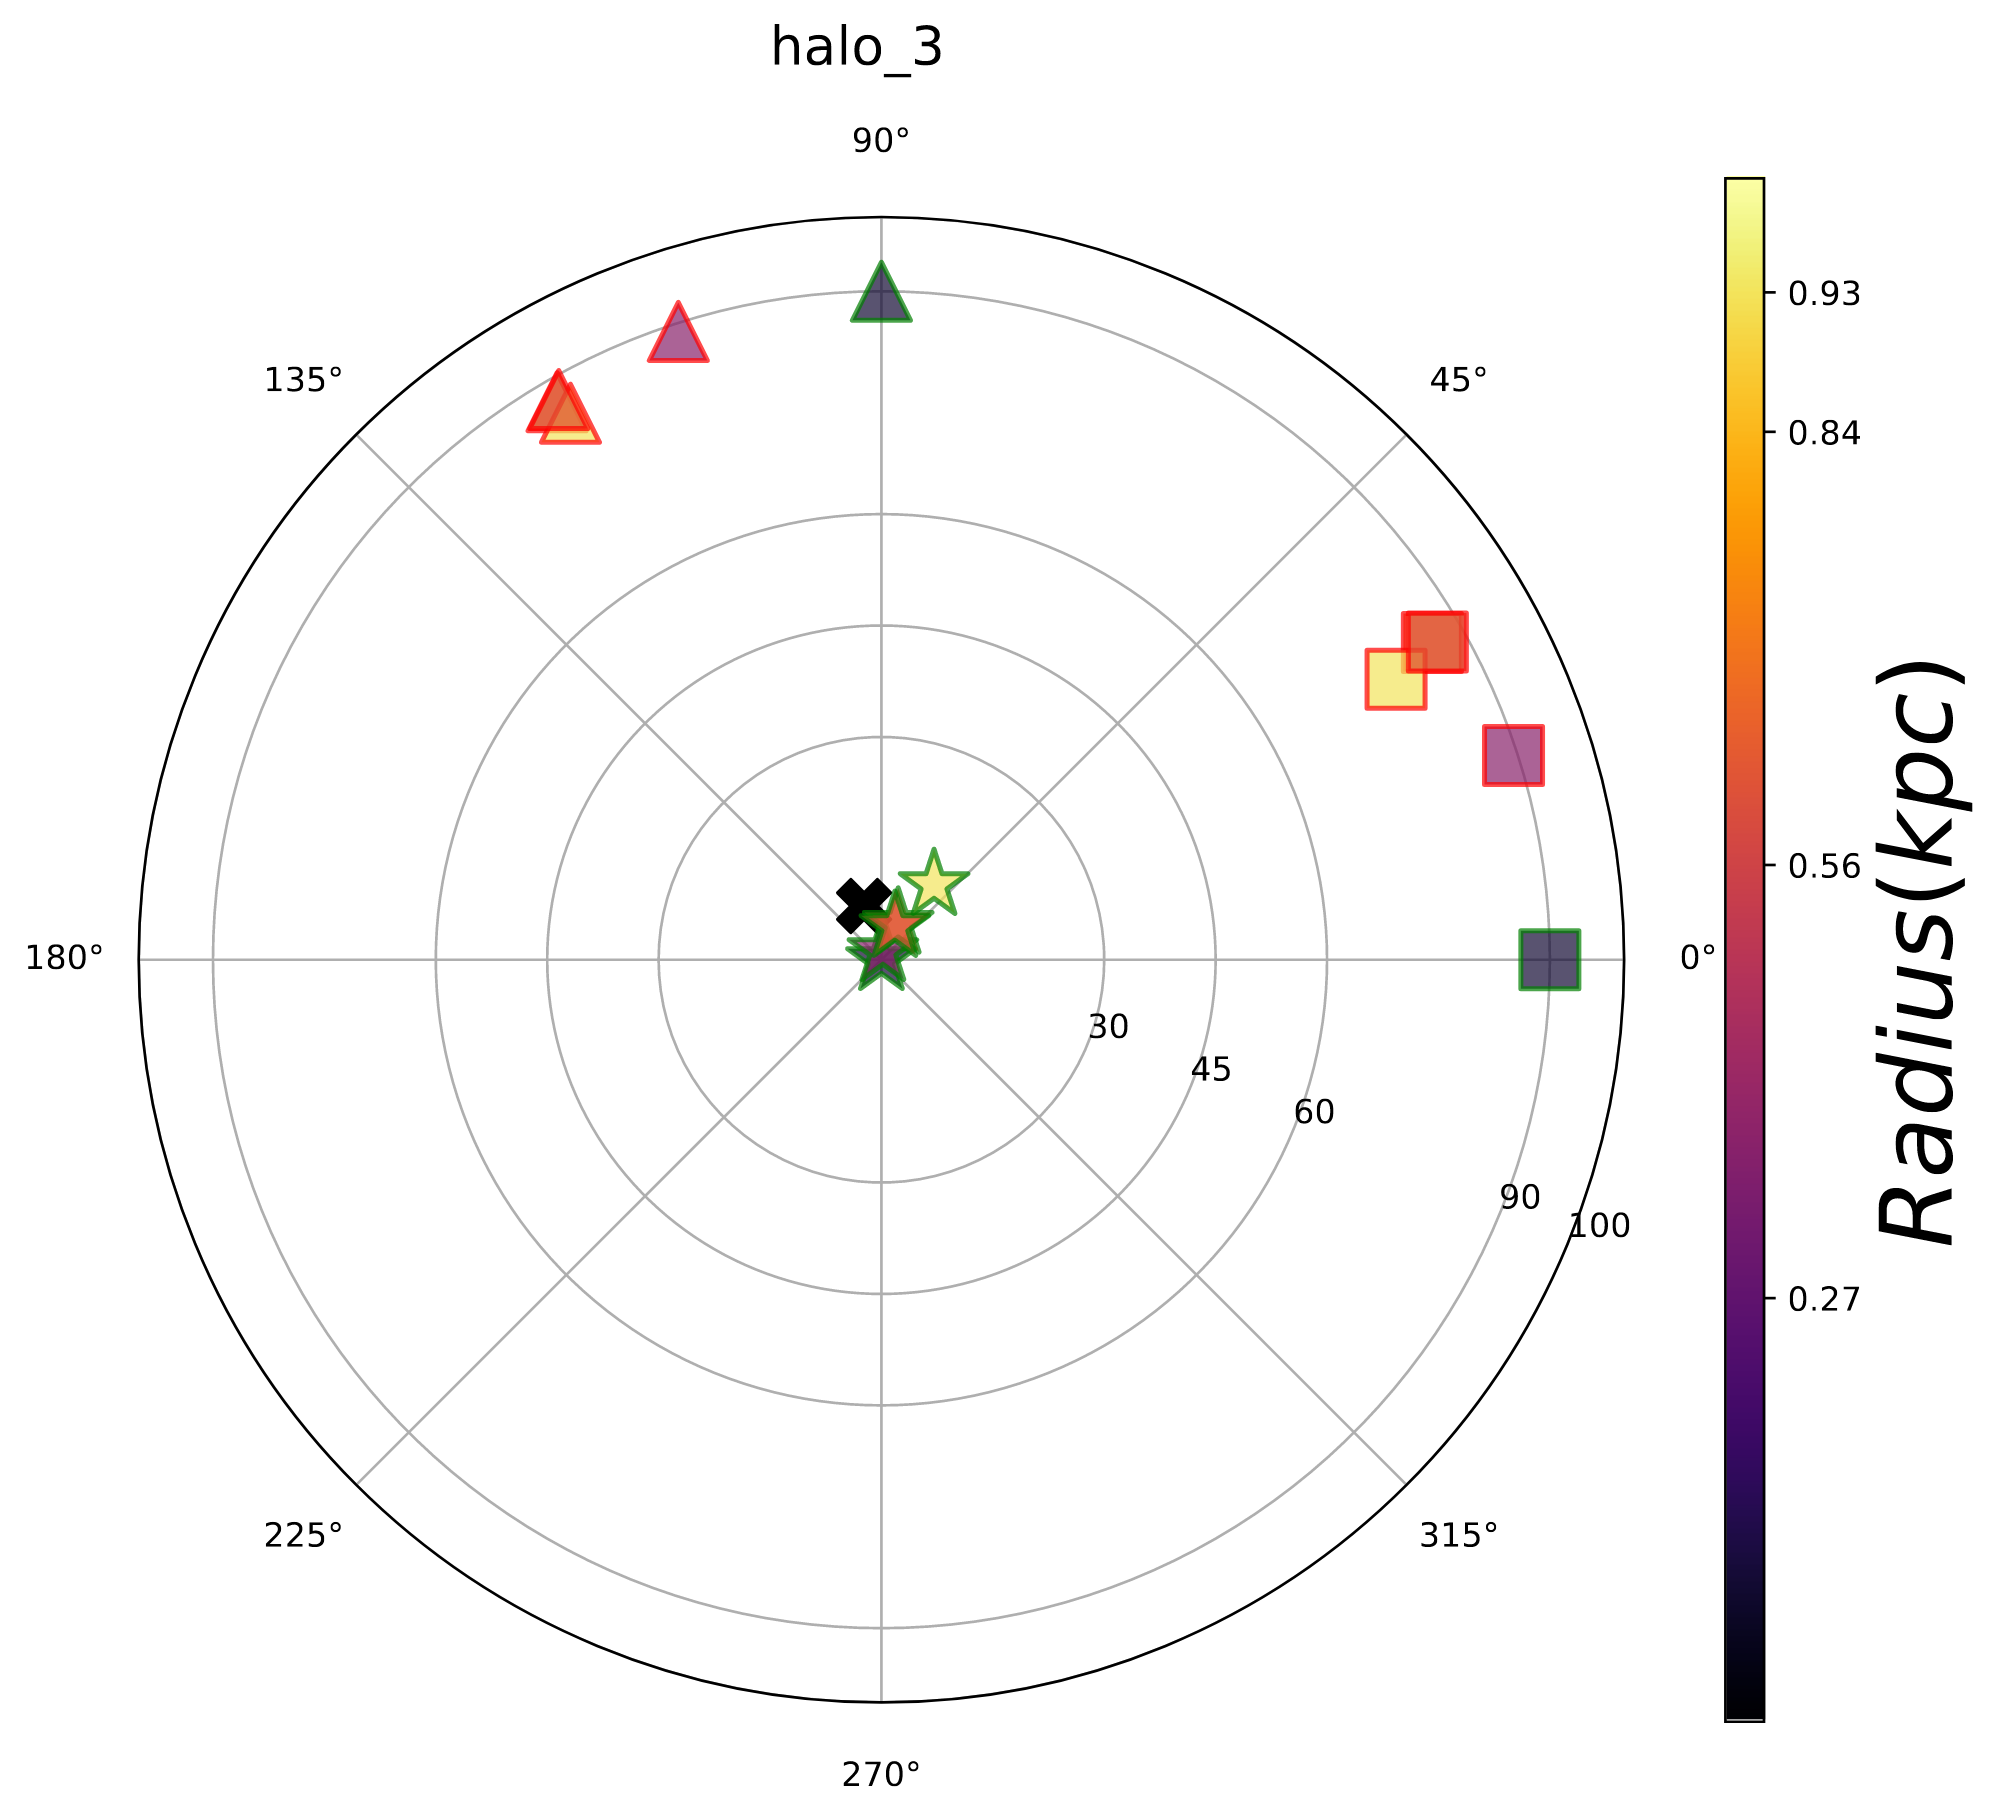
\includegraphics[width=1\columnwidth]{./pics/well_axes.png}}
  \hfill
  \subfloat[Somewhat aligned Axes]{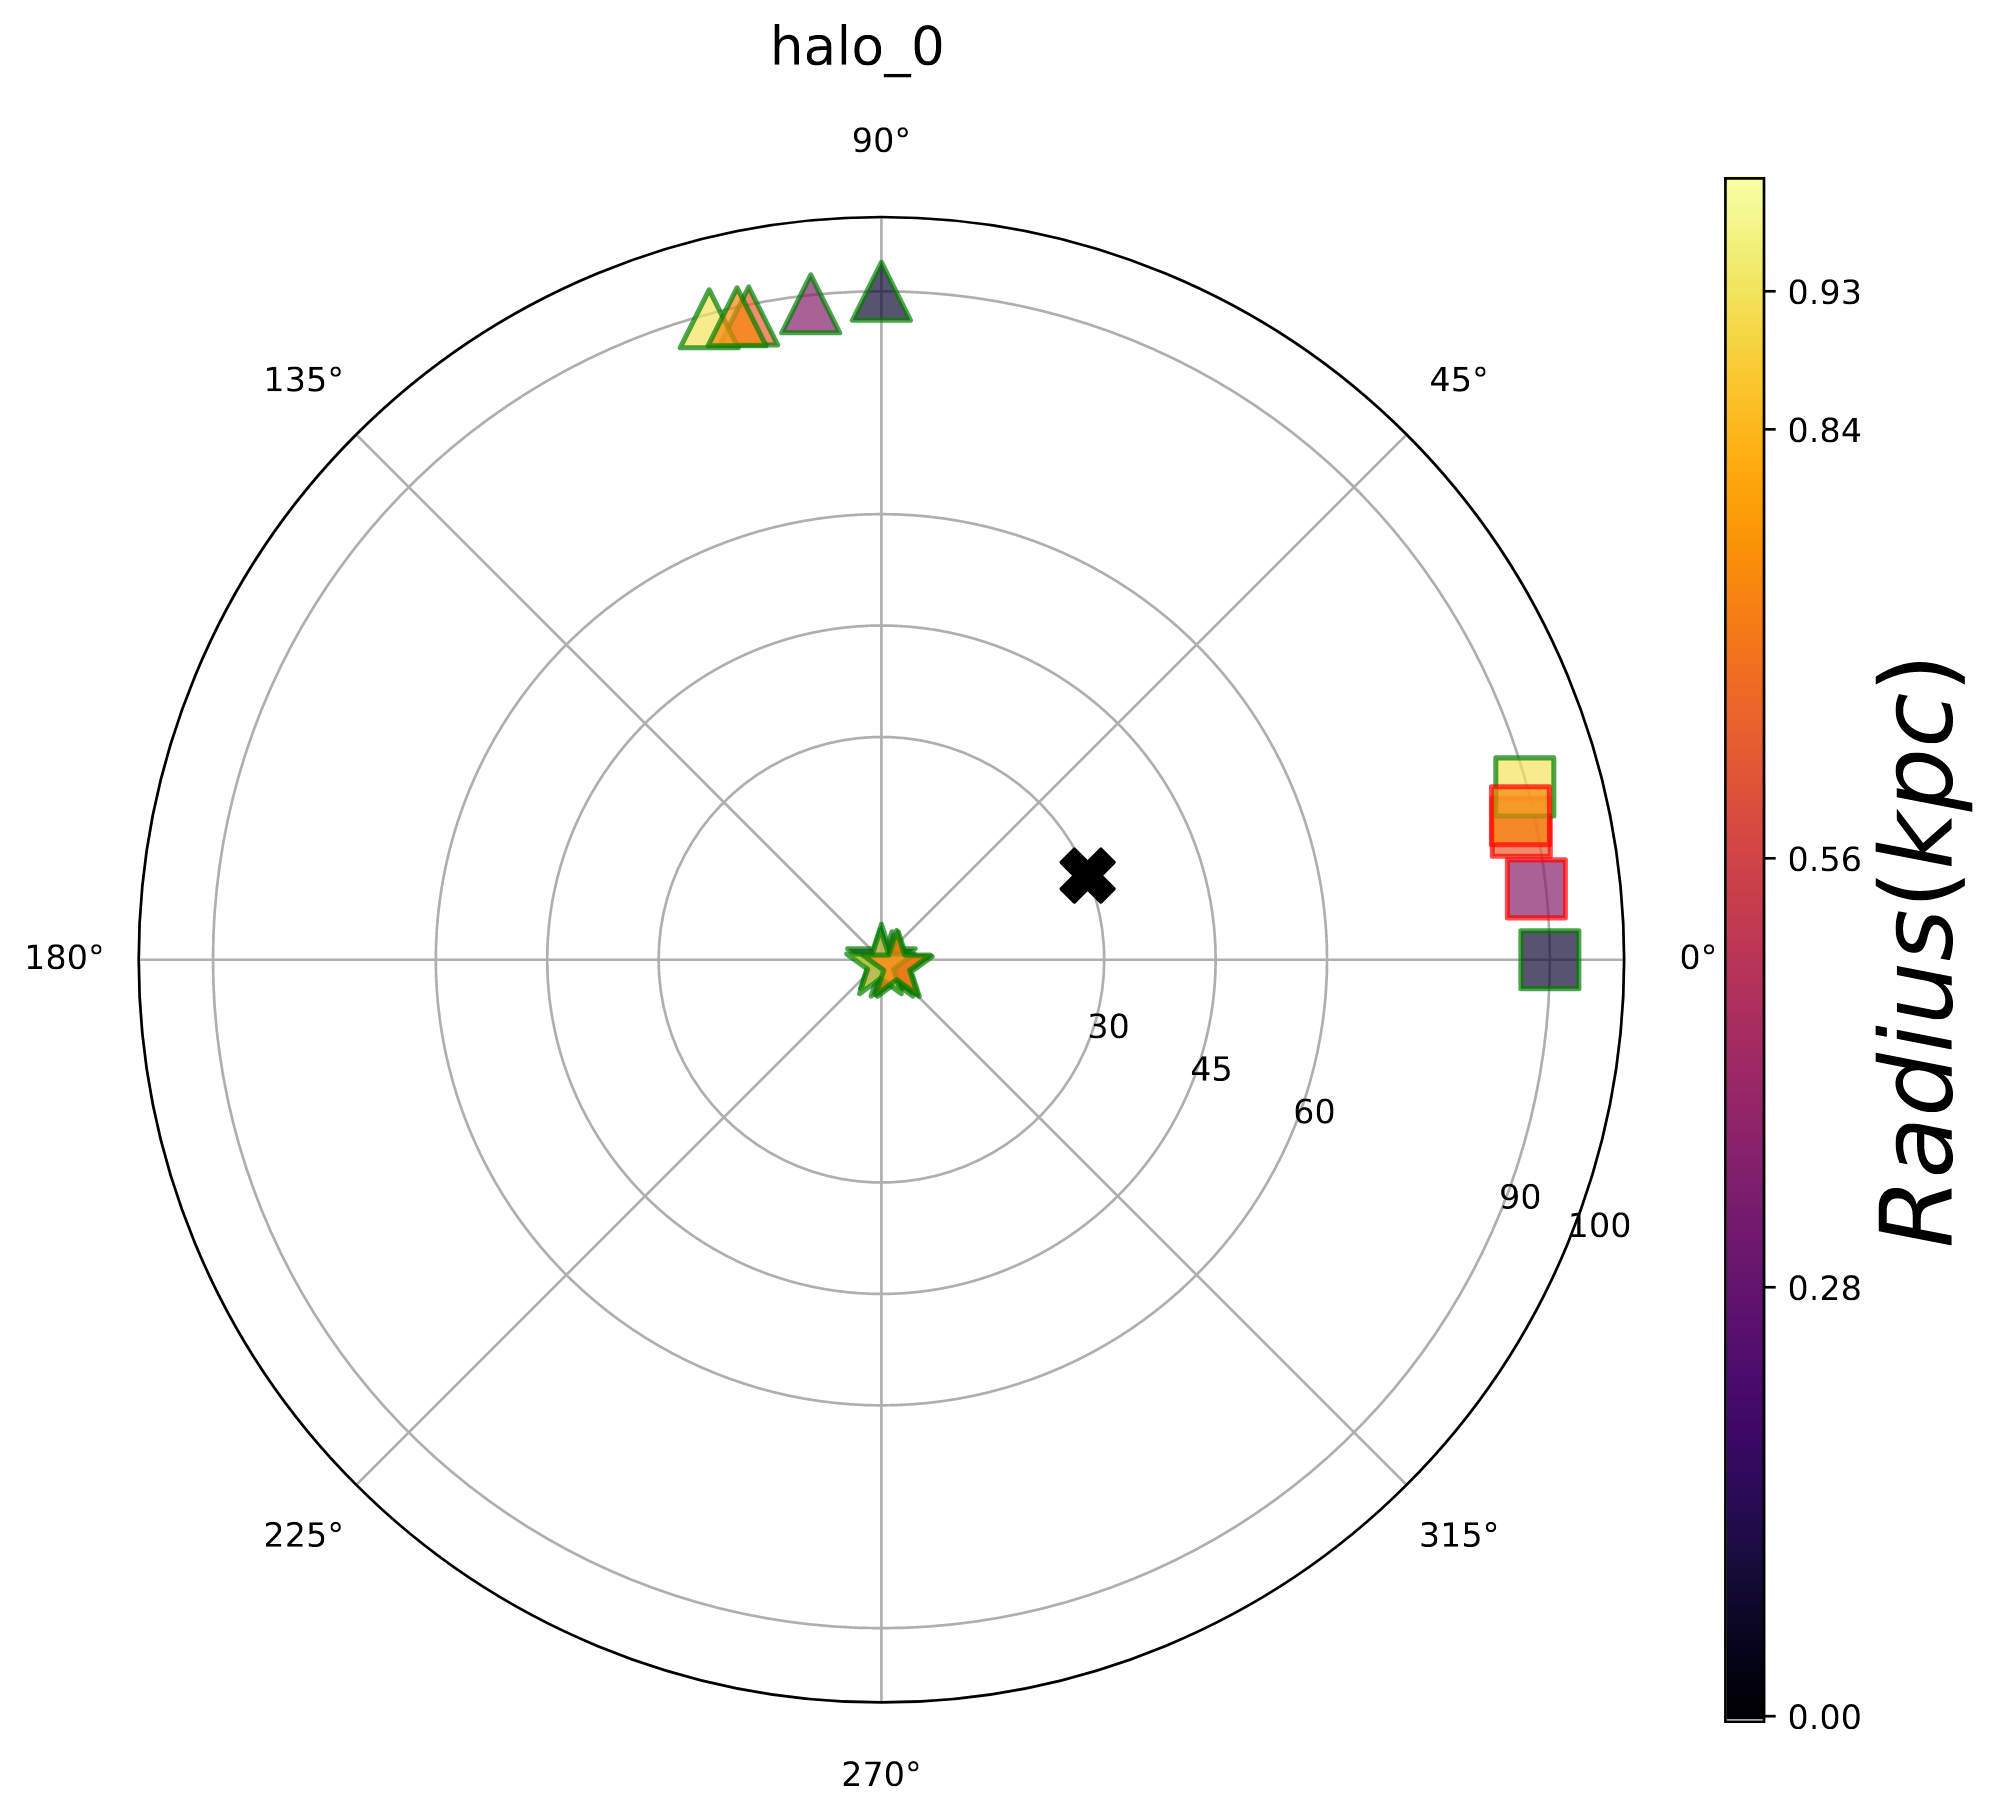
\includegraphics[width=1\columnwidth]{./pics/rotating_axes.png}}
  \hfill
  \subfloat[Chaotic Axes]{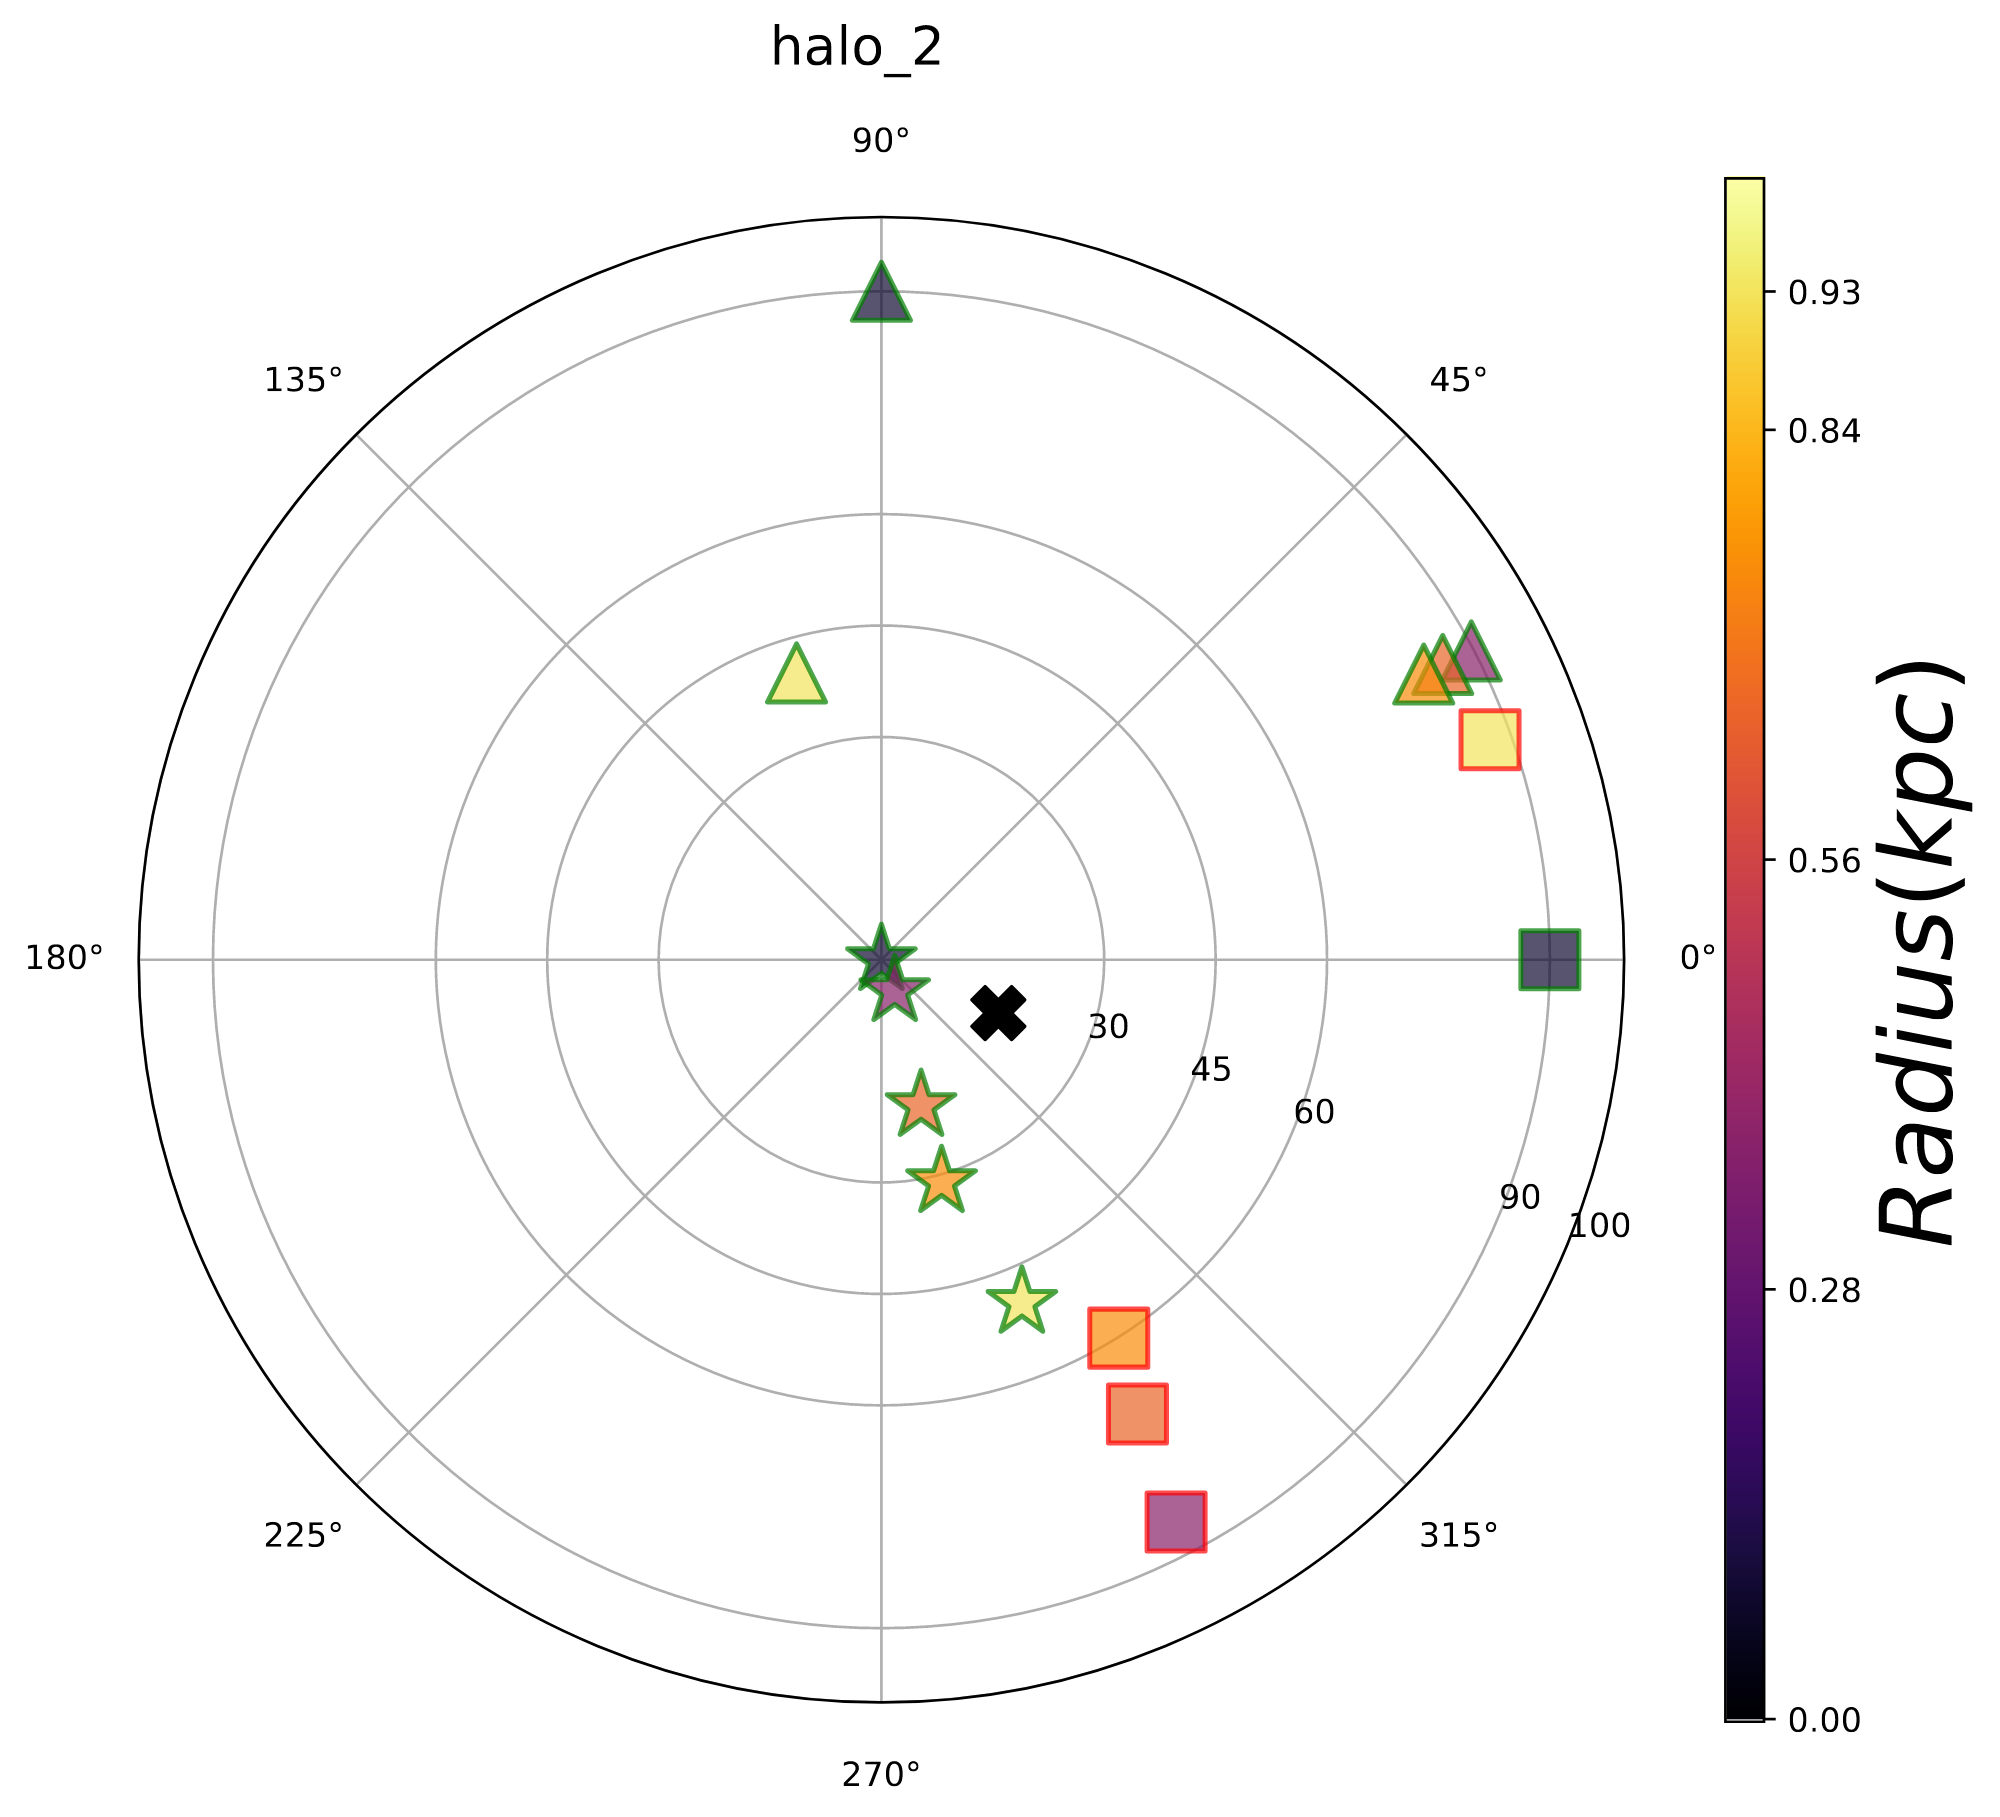
\includegraphics[width=1\columnwidth]{./pics/chaotic_axes.png}}
  \hfill
  \caption{Star: Minor Axis
    Triangle: Medium Axis
    Square: Major Axis
    Color: Radii at which shape was sampled (show radii sampled)
    Contour color: If orientation is above or below in this projection
    Cross (black): Orientation of the stellar disk
    Conclusion: Axes (minor) are not (generally) aligned with the
    stellar disk nor are they usually aligned with each other from
    different radii. We show some cases that may happen.} 
  \label{fig:alignment}
\end{figure}

\textbf{Discussion about the distribution of alignments and their
  evolution in time: Precesion or temporary instabilities?} 



\subsection{Comparison with observational constraints}
To be able to compare our results with observational values, we must relate the calculated quanties with their corresponding isopotential analogue, in which observational constraints are usually presented. For this purpose, we run a simple algorithm to find an approximation of the shape of the isopotential contour. Here, we calculate the mean and standard deviation of the potential over a spherical shell of width equals to $10\%$ of the radius at which it is sampled. Then, we calculate the inertia tensor of particles with potential within $1\sigma$ around the mean potential and calculate its triaxial characterization with the reduced inertia tensor. We repeat the process of calculating the potential mean and standard deviation until convergence is achieved with tolerance of $10^{-4}$. We repeat this process for the different radii from table \ref{tabe:isopotential}. \\

\begin{table}
\setlength{\tabcolsep}{3pt}
\begin{tabular}{l|cccc}
 & $R_{1/8}$& $R_{1/4}$& $R_{1/2}$& $R_1$ \\
\hline \hline
$\bar{q}$&$0.98^{+0.01}_{-0.02}$&$0.97^{+0.01}_{-0.04}$&$0.96^{+0.03}_{-0.06}$&$0.94^{+0.03}_{-0.07}$ \\[0.1cm]
$\bar{s}$&$0.89^{+0.04}_{-0.06}$&$0.88^{+0.04}_{-0.04}$&$0.87^{+0.05}_{-0.05}$&$0.85^{+0.05}_{-0.05}$ \\[0.1cm]
$\bar{T}$&$0.18^{+0.23}_{-0.10}$&$0.36^{+0.19}_{-0.21}$&$0.40^{+0.26}_{-0.20}$&$0.48^{+0.23}_{-0.21}$ \\[0.1cm]
\hline
\end{tabular}
\caption{Median values of isopotential axial ratios $q,s$ and triaxiality parameter $T$ for DM halos in MHD simulations at different radii (columns). }
\label{tabe:isopotential}
\end{table}

As a check of consistency, we compare our new isopotential shape
results with the analytic expression of the
$(1-q_{\phi})\frac{1}{3}(1-q_{\rho})$ \citep{Binney_and_Tremaine_2008}, taking the volume-enclosed axial ratios
as an approximation for the isodensity contour ratios
$q_{\rho}$. Although this analytic expression if meant to be used for
logarithmic axisymmetric halos, it works well as a first approximation
for nearly axisymmetric halos as those produced by our disced
galaxies. We find that the difference between the real and the
analytic isopotential axial ratios is not bigger than $quantity
percent$. With this, we may now present on table
\ref{tabe:isopotential} our observationally-comparable results for MHD
halos at two important radii one corresponding to the approximate
regimes where the MW DM halo is usually constrained. 

Little discussion: Are our results congruent with observations? at
which radii, does the DM halo shape vary that much?. Which models are
favored? 


\subsection{The rounding effect of baryons}

From the previous characterization of radial shapes it is clear that
MHD halos are rounder than DM halos (i.e. axial ratios are bigger) at
every sampled radii. This can be compared on tables \ref{tabe:DM
  table} and \ref{tabe:MHD table} or at the representative example on
figure \ref{fig:DM_MHD}. From there, it is also noticeable that the
rounding effect of baryons is stronger at the disk regime, where the
DM halo is almost perfectly oblate. Furthermore, MHD halos tend
towards more oblate shapes (T < 0.5) despite DM halos tendency towards
more prolate shapes (T>0.5). 

This rounding effect is expected from the gravitational effect of the
flattened axisymmetric galactic disk. It is also reasonable that this
effect is not as strong at $\approx 100$kpc, where the disk potential
is dimmer compared to the DM halo potential. Keeping this in mind, one
would expect that the rounding effect of baryons is related to some
galactic parameters such as its component masses and radii. However,
even for the parameter of highest correlation with this rounding
effect (the baryonic fraction), the relation is not clear nor
conclusive due to the dispersion from galaxy peculiarities. In figure
\ref{fig:Star_Density_effect} we plot the ratios $c/a$ compared to the
baryonic fraction of each galaxy. Although some linear tendency is
suggested qualitatively, the dispersion of the sample is very high to
obtain some conclusive relation. This is an evidence that
adiabatic-contraction models are not realistic as they may neglect
some effects of the galaxy evolution in the whole cosmological
context.  

\begin{figure}
  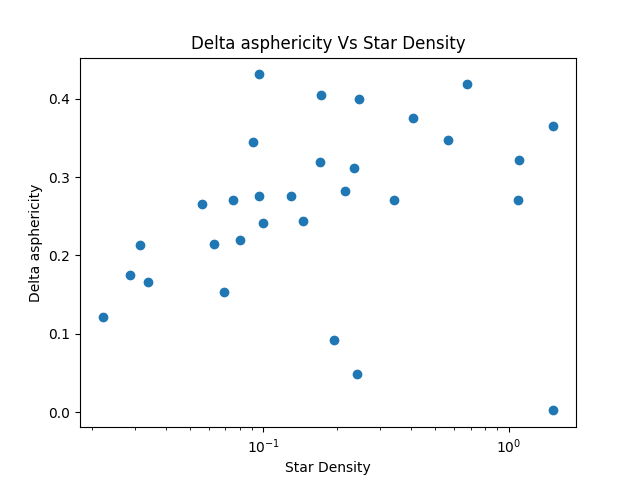
\includegraphics[width=\columnwidth]{./pics/Delta asphericity Vs Star Density.png}
  \caption{Difference in asphericities between MHD and DM shapes Vs
    Star Density of the simulation. Unsure about this graphic. Take
    delta asphericity as the strength of the rounding effect of
    baryons.}  
  \label{fig:Star_Density_effect}
\end{figure}

\textbf{Actually we have not examined the relation of c/a in MHD halos
  with some measure of c/a from the disk, that is something like
  Zdisk/Rdisk. This actually would make more sense from a physical
  point of view: effect of the potential.} 

Although the effect of the baryonic disk on the shape of the DM halo
is a reasonable explanation for the rounding effect, it does not
actually explain the deviation from oblateness of MHD halos at
$r<10$kpc. In other words, if the disk is perfectly axisymmetric,
there must be some source of triaxiality at $r<10$kpc to explain the
low axial ratios. 

\textit{ Talk about source of triaxiality at the inner parts of the
  halos (bar?). This source of triaxiality at the inner parts explains
  why the axial ratios are $\approx 0.95$ and not exactly $1$. We
  should also discuss that the decrease in the axial ratios for bigger
  radii may actually be bigger/steeper but it is dimmed by the
  contribution of inner parts.} 
%
%\begin{figure}
%  \centering
%  \subfloat[Level4 MHD Vs DM at inner regions]{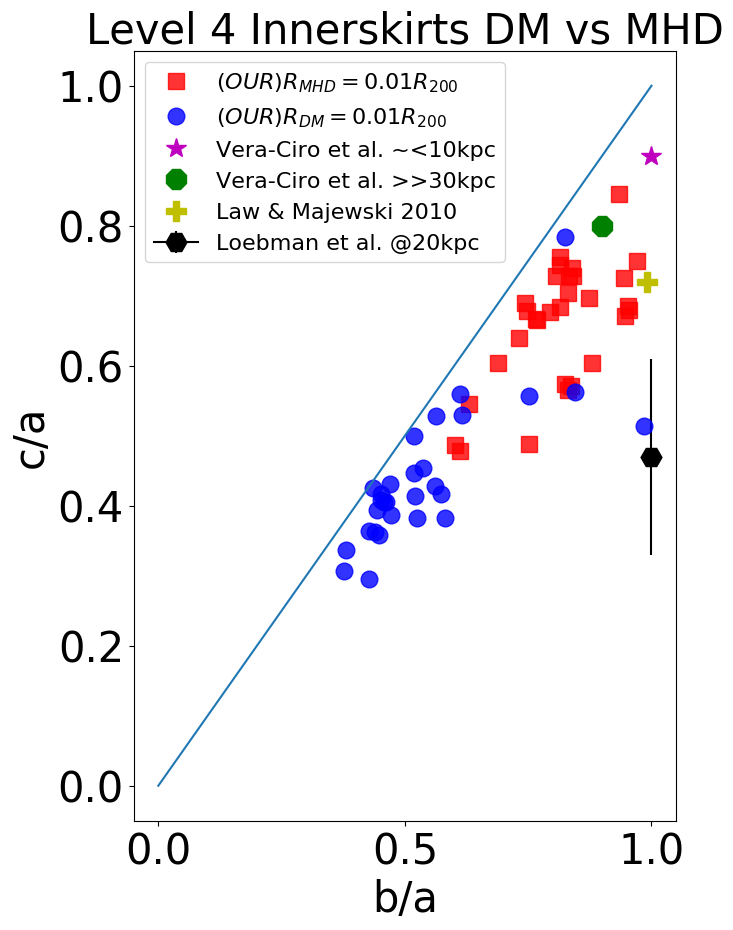
\includegraphics[width=0.5\columnwidth]{./pics/Triaxial_Plane/Triaxiality_Inner_lvl4.png}}
%  \hfill
%  \subfloat[Level4 MHD Vs DM at outer regions]{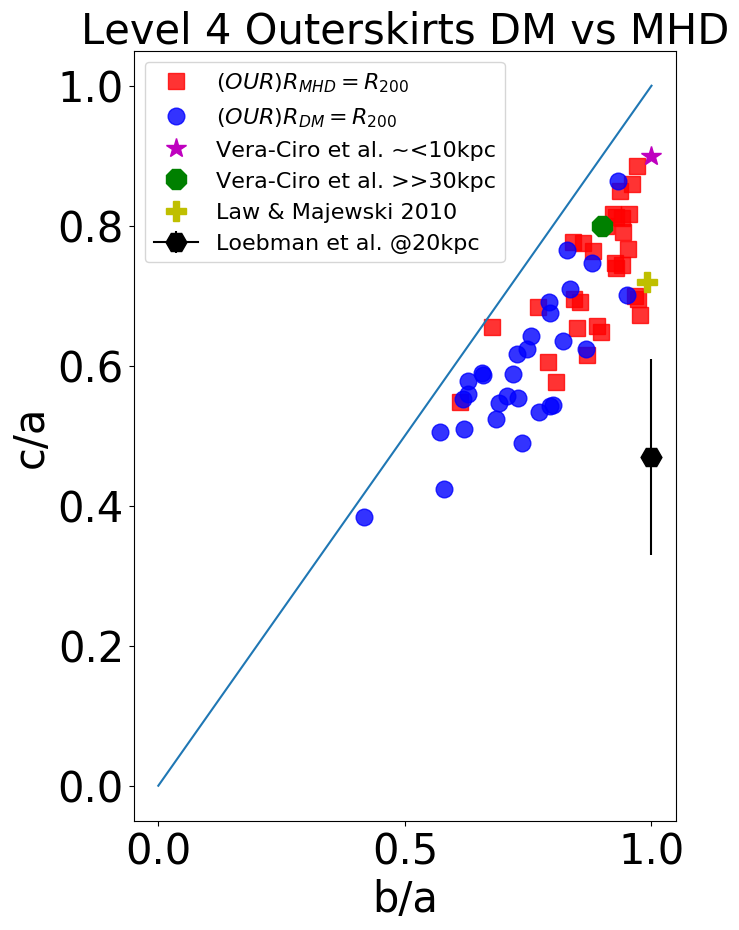
\includegraphics[width=0.5\columnwidth]{./pics/Triaxial_Plane/Triaxiality_Outter_lvl4.png}}
%  \hfill
%  \caption{Axial ratios as shown on $c/a$ Vs $b/a$. Each dot represents a halo shape at some radius. Some observational constraints are plotted alongside our results. Here, dots are clustered, proving the general tendence of halos to get rounder on the outer parts.(Optimize space. caption replaces title.  Present constraints representation of density)}
%  \label{fig:Triaxiality_Inner_Outer}
%\end{figure}


\section{Conclusions}

\section{Discussion}

\section*{Acknowledgements}
This project has received funding from the European Union’s Horizon
2020 Research and Innovation Programme under the Marie
Sk\l{}odowska-Curie grant agreement No 734374. 

 \bibliographystyle{mnras}
 \bibliography{references}
\end{document}
